\chapter{Supplemental Information}
\label{chap:appendix}
\thispagestyle{empty}

%%%%%%%%%%%%%%%%%%%%%%%%%%%%%%%%%%%%%%%%%%%%%%%%%%%%
%%%%%%%%%%%%%%%%%%%%%%%%%%%%%%%%%%%%%%%%%%%%%%%%%%%%
%%%%%%%%%%%%%%%%%%%%%%%%%%%%%%%%%%%%%%%%%%%%%%%%%%%%

\section{List of Chemicals}
\label{sup:LoChemicals}

\begin{table}[htbp]
	\centering
	\caption[List of Compounds]{List of chemical compounds used during the course of this study.}
	\label{tbl:LoCompounds}
	\begin{tabular}{llrrl}
		\toprule
		Chemical				&Chemical 			&CAS \#		&Molec.	&Source	\\ 
		Name				&Formula				&			&Weight	&		\\\midrule
		Lead(II) hexafluoro- 		&\ce{Pb(C5O2HF6)2}	&19648-88-5	&621.29	&Strem Chemicals, Inc.\\	
		acetylacetonate		\\
		Bis(2,2,6,6-tetramethyl	&\ce{Pb(C11H19O2)2}	&21319-43-7	&573.50	&Strem Chemicals, Inc.\\
		-3,5-heptanedionato)\\
		Lead(II)\\
		Titanium(IV)			&\ce{Ti[OCH(CH3)2]4}	&546-68-9	&284.25	&Strem Chemicals, Inc.\\
		i-propoxide\\\midrule
		Isopropyl Alcohol (IPA)	&\ce{(CH3)2CHOH}		&67-63-0		&60.10	&Alfa Aesar\\
		Acetone				&\ce{C3H6O}			&67-64-1		&58.08	&Alfa Aesar\\
		Buffered Hydrofluoric	&\ce{NH4F}-\ce{HF}		&7664-39-3	&N/A		&Alfa Aesar\\
		Acid (BHF)			&					&\& 12125-01-8\\
		Ozone				&\ce{O3}				&10028-15-6	&48.00	&\\
		\bottomrule
	\end{tabular}
\end{table}

\clearpage

%%%%%%%%%%%%%%%%%%%%%%%%%%%%%%%%%%%%%%%%%%%%%%%%%%%%
%%%%%%%%%%%%%%%%%%%%%%%%%%%%%%%%%%%%%%%%%%%%%%%%%%%%
%%%%%%%%%%%%%%%%%%%%%%%%%%%%%%%%%%%%%%%%%%%%%%%%%%%%

%\begin{landscape}
%\section{List of Samples}
%\label{sup:LoSamples}

%{
%\begin{longtable}{c c c c c c c c c}
%	\caption[List of Samples]{A list of samples used during the course of this project.%
%	\label{tbl:LoSamples}}\\
%	\toprule
%	&&&&&\multicolumn{3}{c}{Annealing}&\\ \cmidrule{6-8}
%	Temp.		&Run \#	&Pb:Ti	 	&Cycles 	&Subs. 	&Type	&Temp. 		&Time &XRD\\ 
%	(\degC{})		&		&Ratio		&		&Type	&		&(\degC{})	&(min) &\\ \midrule%
%	\endfirsthead
%	\caption[]{A list of samples used during the course of this project.}\\
%	\toprule
%	&&&&&\multicolumn{3}{c}{Annealing}&\\ \cmidrule{6-8}
%	Temp.		&Run \#	&Pb:Ti	 	&Cycles 	&Subs. 	&Type	&Temp. 		&Time &XRD\\ 
%	(\degC{})		&		&Ratio		&		&Type	&		&(\degC{})	&(min) &\\ \midrule%
%	\endhead
%	200	&3		&1:1		&250	&Si		&None	&N/A		&N/A		&No\\
%		&2		&1:2		&250	&Si		&None	&N/A		&N/A		&No\\
%		&30		&3:1		&160	&Si		&None	&N/A		&N/A		&No\\
%		&		&		&		&Pt-Si	&None	&N/A		&N/A		&No\\ \midrule
%	250	&0		&1:1		&625	&Si		&Oven	&650	&120	&Yes\\
%		&		&		&		&		&Oven	&900	&120	&Yes\\
%		&		&		&		&		&RTA	&900	&10		&No\\
%		&1		&1:1		&475	&Si		&None	&N/A		&N/A		&No\\
%		&6		&1:2		&250	&Si		&None 	&N/A		&N/A		&No\\
%		&13		&3:1		&250	&Si		&None 	&N/A		&N/A		&No\\
%		&16		&3:1		&150	&Si		&RTA	&650	&1		&No\\
%		&19		&3:1		&100	&Si		&None 	&N/A		&N/A		&No\\
%		&		&		&		&Pt-Si	&None 	&N/A		&N/A		&No\\
%		&20		&3:1		&200	&Si		&None 	&N/A		&N/A		&No\\
%		&		&		&		&Pt-Si	&Oven	&650	&90		&Yes\\
%		&21		&3:1		&150	&Si		&None 	&N/A		&N/A		&No\\
%		&		&		&		&Pt-Si	&Oven	&650	&90		&No\\ \\
%		&22		&3:1		&150	&Si		&None 	&N/A		&N/A		&No\\
%		&		&		&		&Pt-Si	&Oven	&650	&90		&Yes\\
%		&23		&3:1		&200	&Si		&None 	&N/A		&N/A		&No\\
%		&		&		&		&Pt-Si	&Oven	&650	&90		&Yes\\
%		&28		&3:1		&120	&STO	&Oven	&650	&90		&Yes\\
%	\bottomrule
%\end{longtable}}
%\clearpage
%%%%%%%%%%%%%%%%%%%%%%%%%%%%%%%%%%%%%%%%%%%%%%%%%%%%
%%%%%%%%%%%%%%%%%%%%%%%%%%%%%%%%%%%%%%%%%%%%%%%%%%%%
%%%%%%%%%%%%%%%%%%%%%%%%%%%%%%%%%%%%%%%%%%%%%%%%%%%%
%\begin{landscape}
\section{ALD Reactor Diagram}
\label{sup:ALD-design}

\begin{figure}[htb]
   \centering
   \subfloat[Photograph][Photograph]{%
   	\label{fig:S100-photo}%
	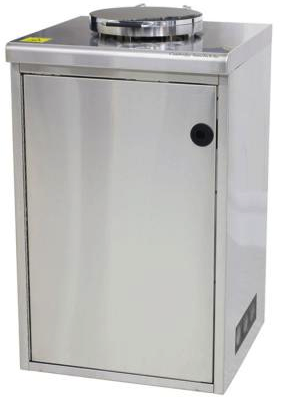
\includegraphics[height=8cm]{./Figures/Appendix/ALD-schematic/savannah-s100}%
	} 
	\hspace{1cm}
  \subfloat[Schematic Diagram][Schematic Diagram]{%
   	\label{fig:S100-schematic}%
	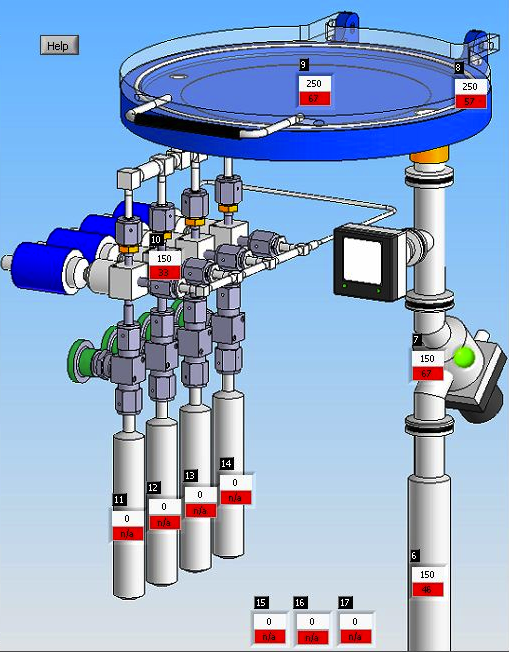
\includegraphics[height=8cm]{./Figures/Appendix/ALD-schematic/savannah-schematic}%
	} 	
   \caption[Cambridge NanoTech, inc. S100 ALD System]%
   		{Cambridge NanoTech, inc. Savannah S100 ALD reactor. Precursors are stored in heated cylinders, flow up to the reaction zone, and byproducts are pumped out of the vacuum line on the right side. Each zone can be individually temperature controlled.}
   \label{fig:S100}
\end{figure}

\clearpage
%
%\begin{figure}[htbp]
%	\begin{center}
%		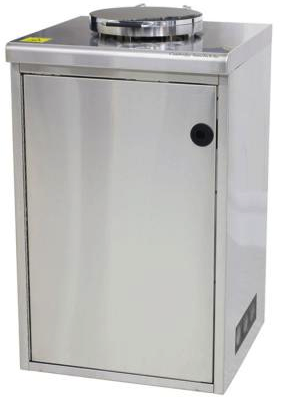
\includegraphics[width=0.5\textwidth]{./Figures/Appendix/ALD-schematic/savannah-s100}
%		\caption[Photograph of S100 ALD Reactor]{Photograph of the Cambridge NanoTech, inc. %
%				Savannah S100 ALD reactor}
%		\label{fig:S100-photo}
%	\end{center}
%\end{figure}
%
%\begin{figure}[htbp]
%	\begin{center}
%		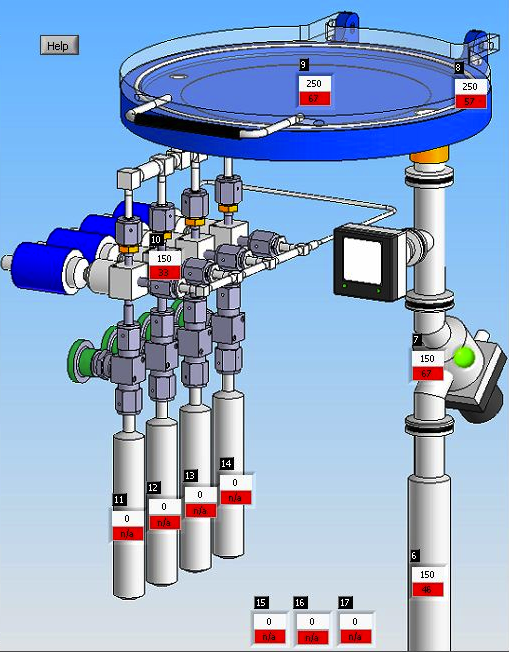
\includegraphics[width=0.85\textwidth]{./Figures/Appendix/ALD-schematic/savannah-schematic}
%		\caption[Diagram of S100 ALD Reactor]{Diagram of the Cambridge NanoTech, inc. %
%				Savannah S100 ALD reactor. Precursors are stored in heated cylinders, flow up to the reaction zone, and byproducts are pumped out of the vacuum line on the right side. Each zone can be individually temperature controlled. }
%		\label{fig:S100-schematic}
%	\end{center}
%\end{figure}


%\end{landscape}
%%%%%%%%%%%%%%%%%%%%%%%%%%%%%%%%%%%%%%%%%%%%%%%%%%%%
%%%%%%%%%%%%%%%%%%%%%%%%%%%%%%%%%%%%%%%%%%%%%%%%%%%%
%%%%%%%%%%%%%%%%%%%%%%%%%%%%%%%%%%%%%%%%%%%%%%%%%%%%

%\section{Recipes for S100 ALD System}
%\label{sup:recipes}
%
%Should recipes be provided? They'd be rather specific to the instrumentation, and some of the recipes are provided by CNT (able to freely publish them?). This section would be trivial to construct, or remove entirely. 
%%
%%Provided in this section are recipes for the deposition of materials in the \ce{Pb_{x}Ti_{y}O_{z}} system. 
%%Some of these recipes (\ce{HfO2}, \ce{Pt}, and \ce{TiO2}) were provided courtesy of Cambridge NanoTech, inc.\cite{CNT-web} 
%%
%\clearpage
%%%%%%%%%%%%%%%%%%%%%%%%%%%%%%%%%%%%%%%%%%%%%%%%%%%%
%%%%%%%%%%%%%%%%%%%%%%%%%%%%%%%%%%%%%%%%%%%%%%%%%%%%
%%%%%%%%%%%%%%%%%%%%%%%%%%%%%%%%%%%%%%%%%%%%%%%%%%%%

%\section{Thermal Analysis Results}
%\label{sup:Thermal-Results}
%
%\subsection{Thermogravimetric Analysis}
%\label{sup:Thermal-Results-TGA}
%
%%\begin{figure}[htbp]
%%   \centering
%%   \subfloat[Mass vs. Temperature][Mass vs. Temperature]{%
%%   	\label{fig:TGA-HFAc-Weight}%
%%	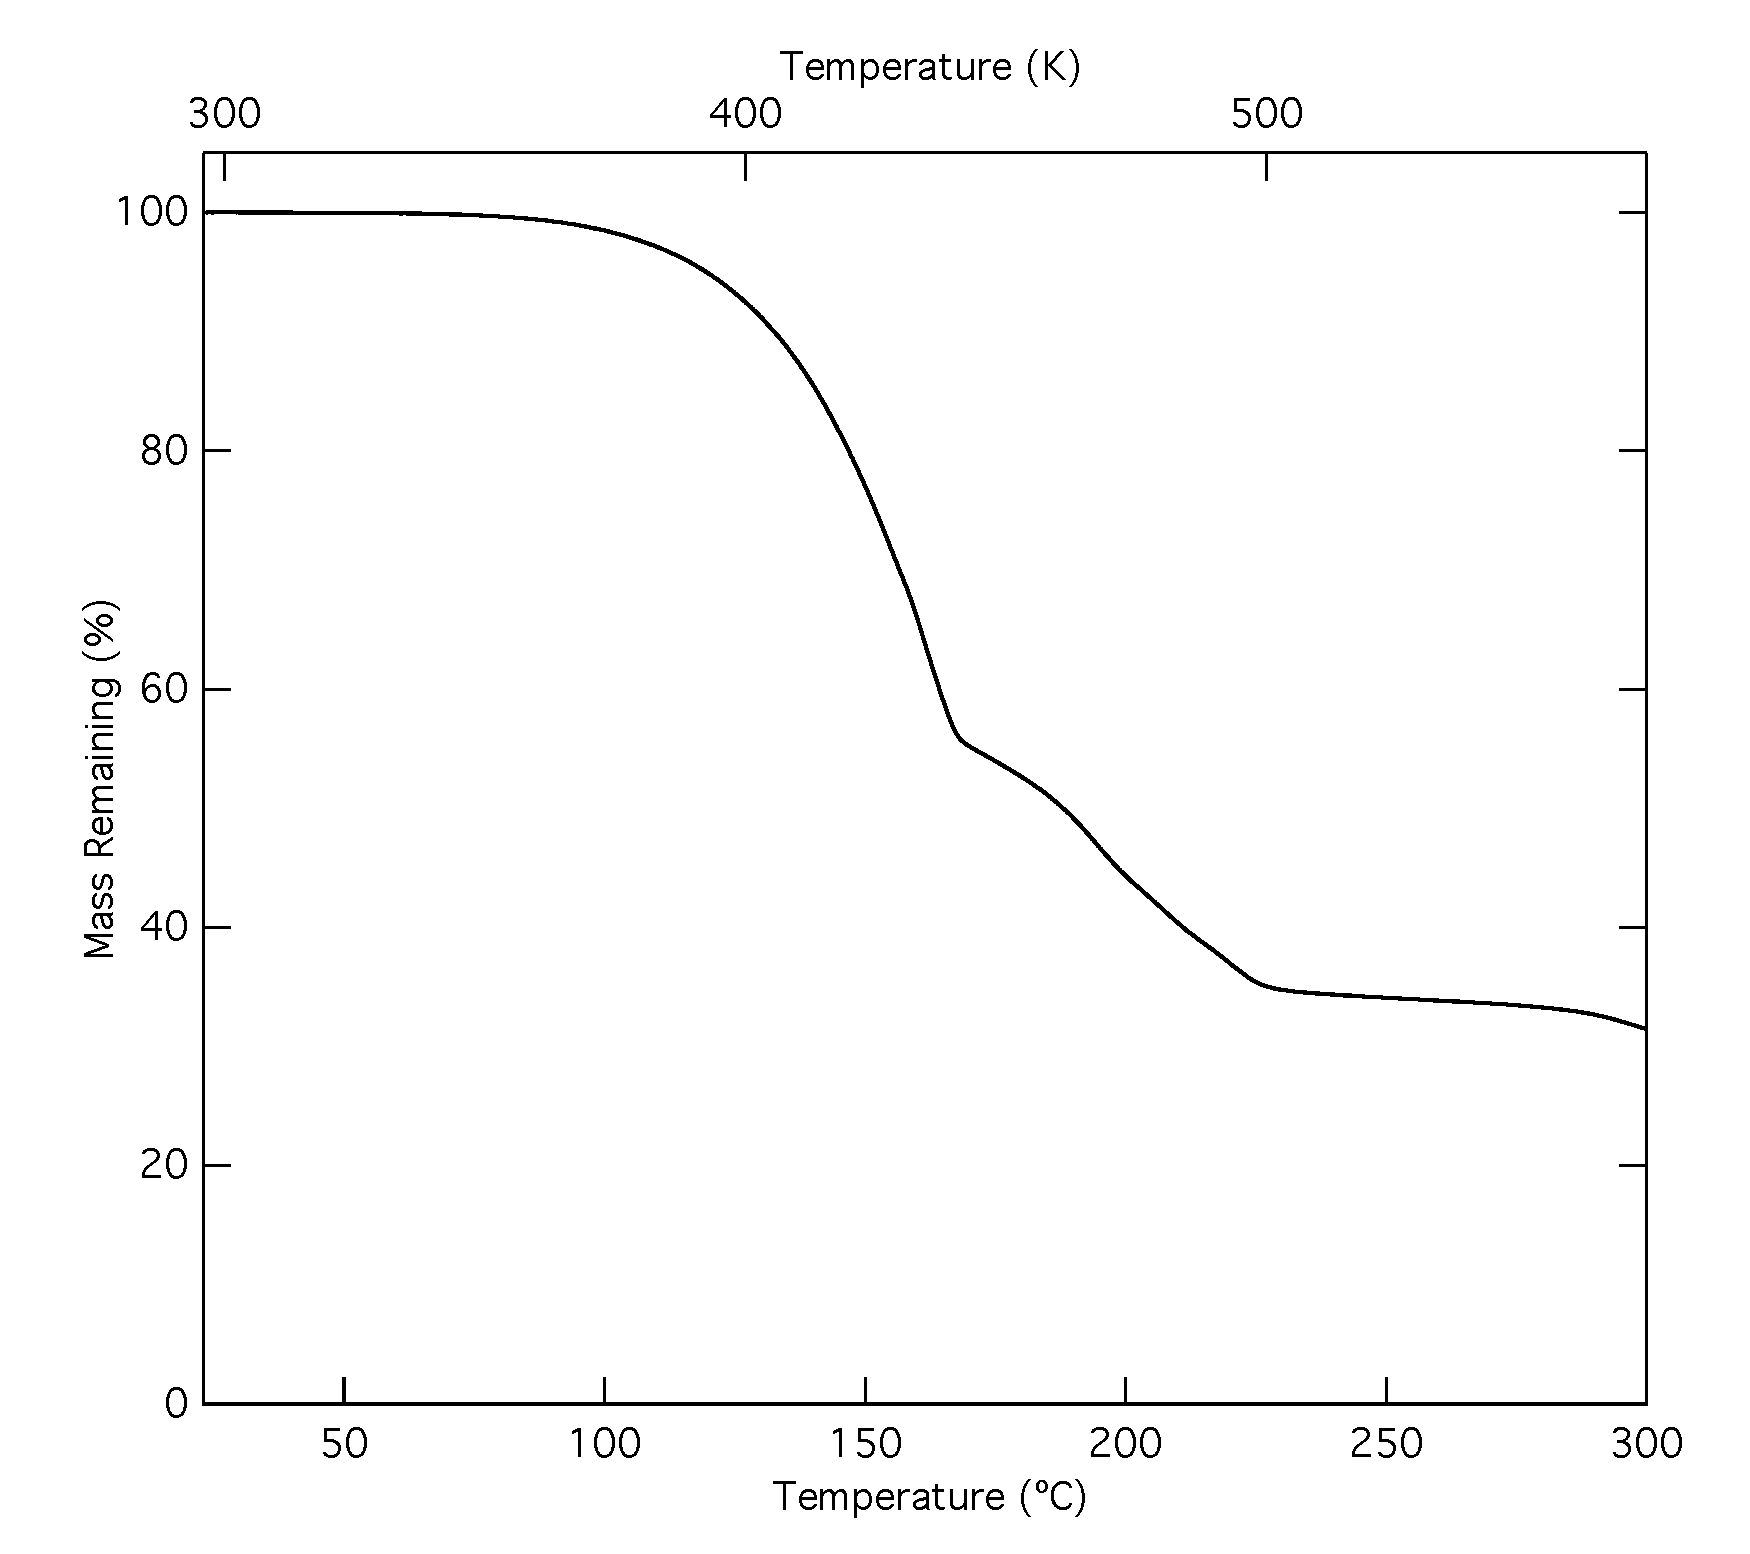
\includegraphics[width=0.5\textwidth]{./Figures/Appendix/Thermal-Analysis/TGA/HFAc-Weight}%
%%	} \\
%%%	\hspace{1cm}
%%  \subfloat[Derivative of Mass vs. Temperature][Derivative of Mass vs. Temperature]{%
%%   	\label{fig:TGA-HFAc-DWeight}%
%%	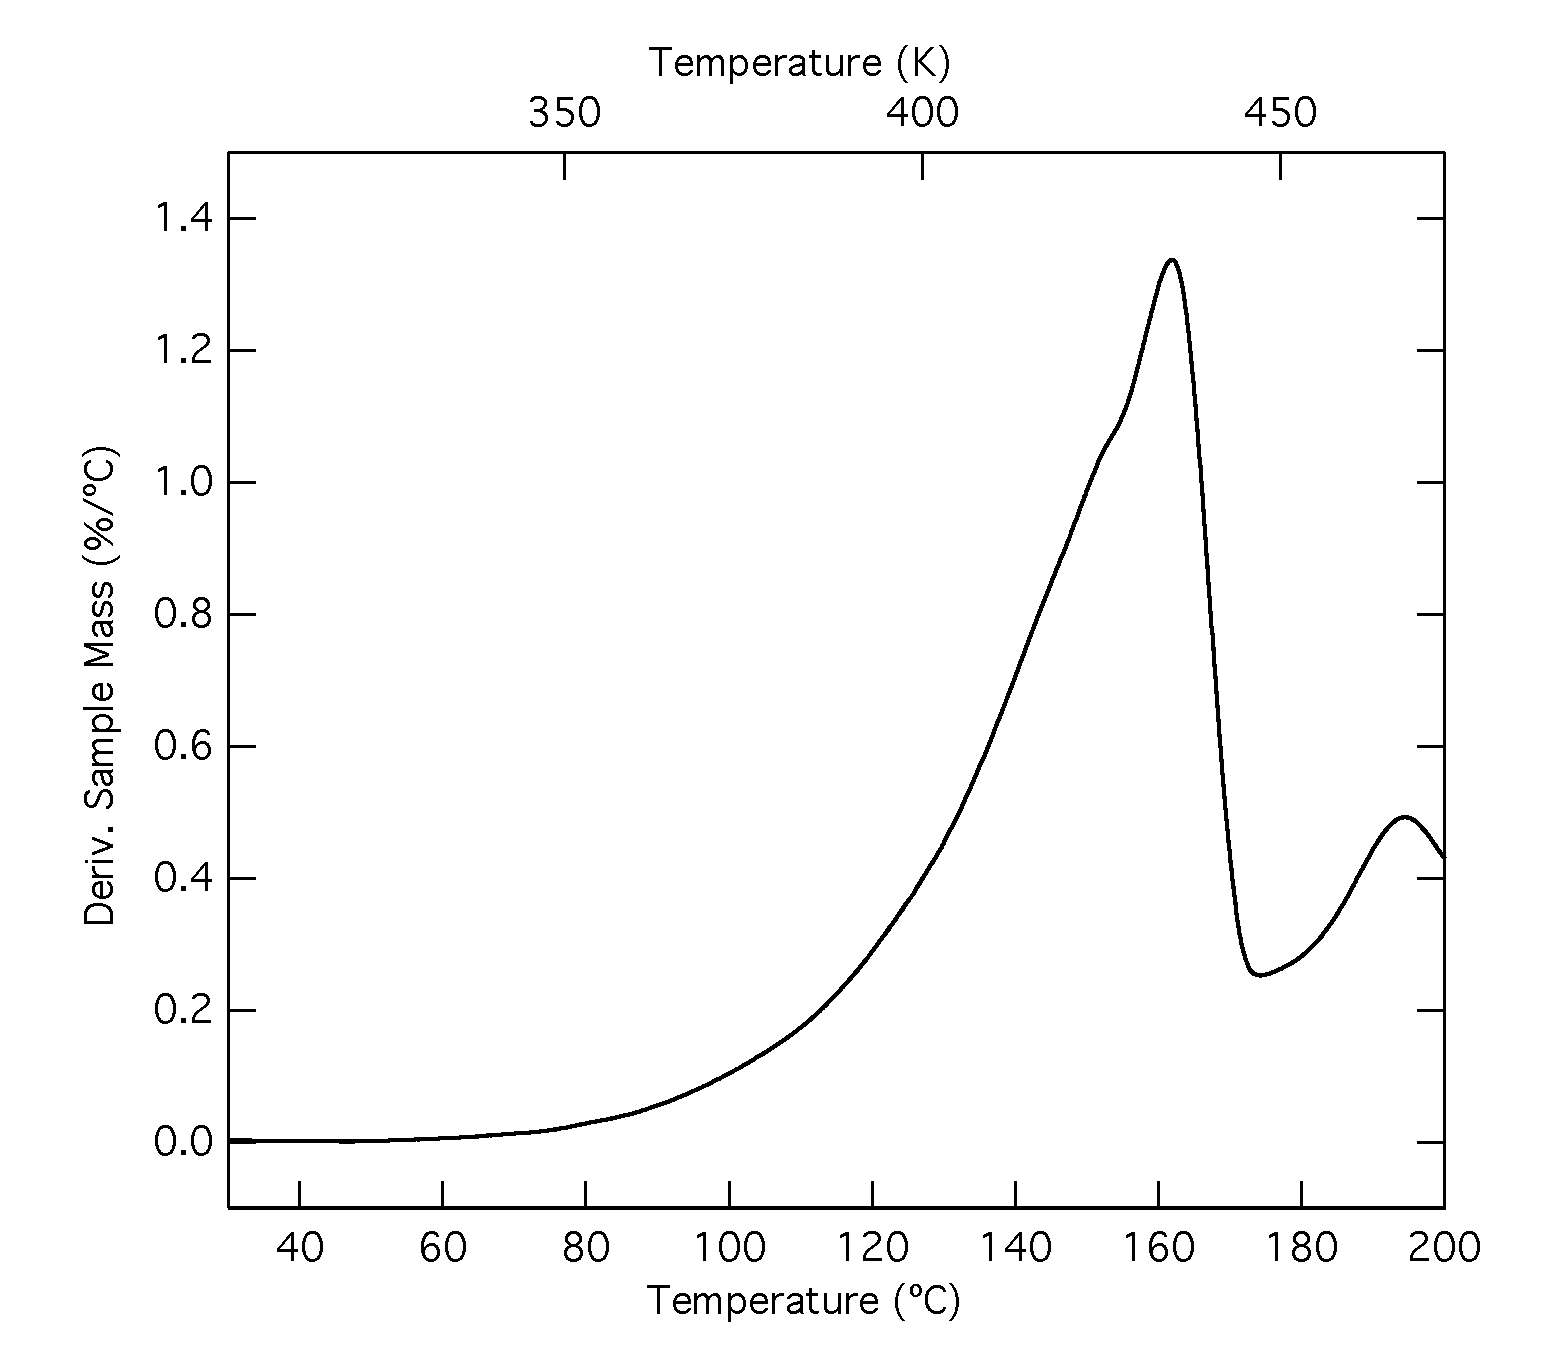
\includegraphics[width=0.5\textwidth]{./Figures/Appendix/Thermal-Analysis/TGA/HFAc-DWeight}%
%%	} 	
%%   \caption[TGA Results for Pb(HFAc)$_{2}$ Precursor]%
%%   		{Plots of the results from TGA experiments on Pb(HFAc)$_{2}$. The plot shown in (a) gives the raw %
%%		data showing the current mass as a function of temperature. (b) gives the same data, transformed %
%%		to show the derivative of mass. Thus (b) shows the rate of mass loss at a given temperature. Initial %
%%		sample mass: 6.092 mg}
%%   \label{fig:TGA-HFAc}
%%\end{figure}
%%
%%\begin{figure}[htbp]
%%   \centering
%%   \subfloat[Mass vs. Temperature][Mass vs. Temperature]{%
%%   	\label{fig:TGA-TMHD-Weight}%
%%	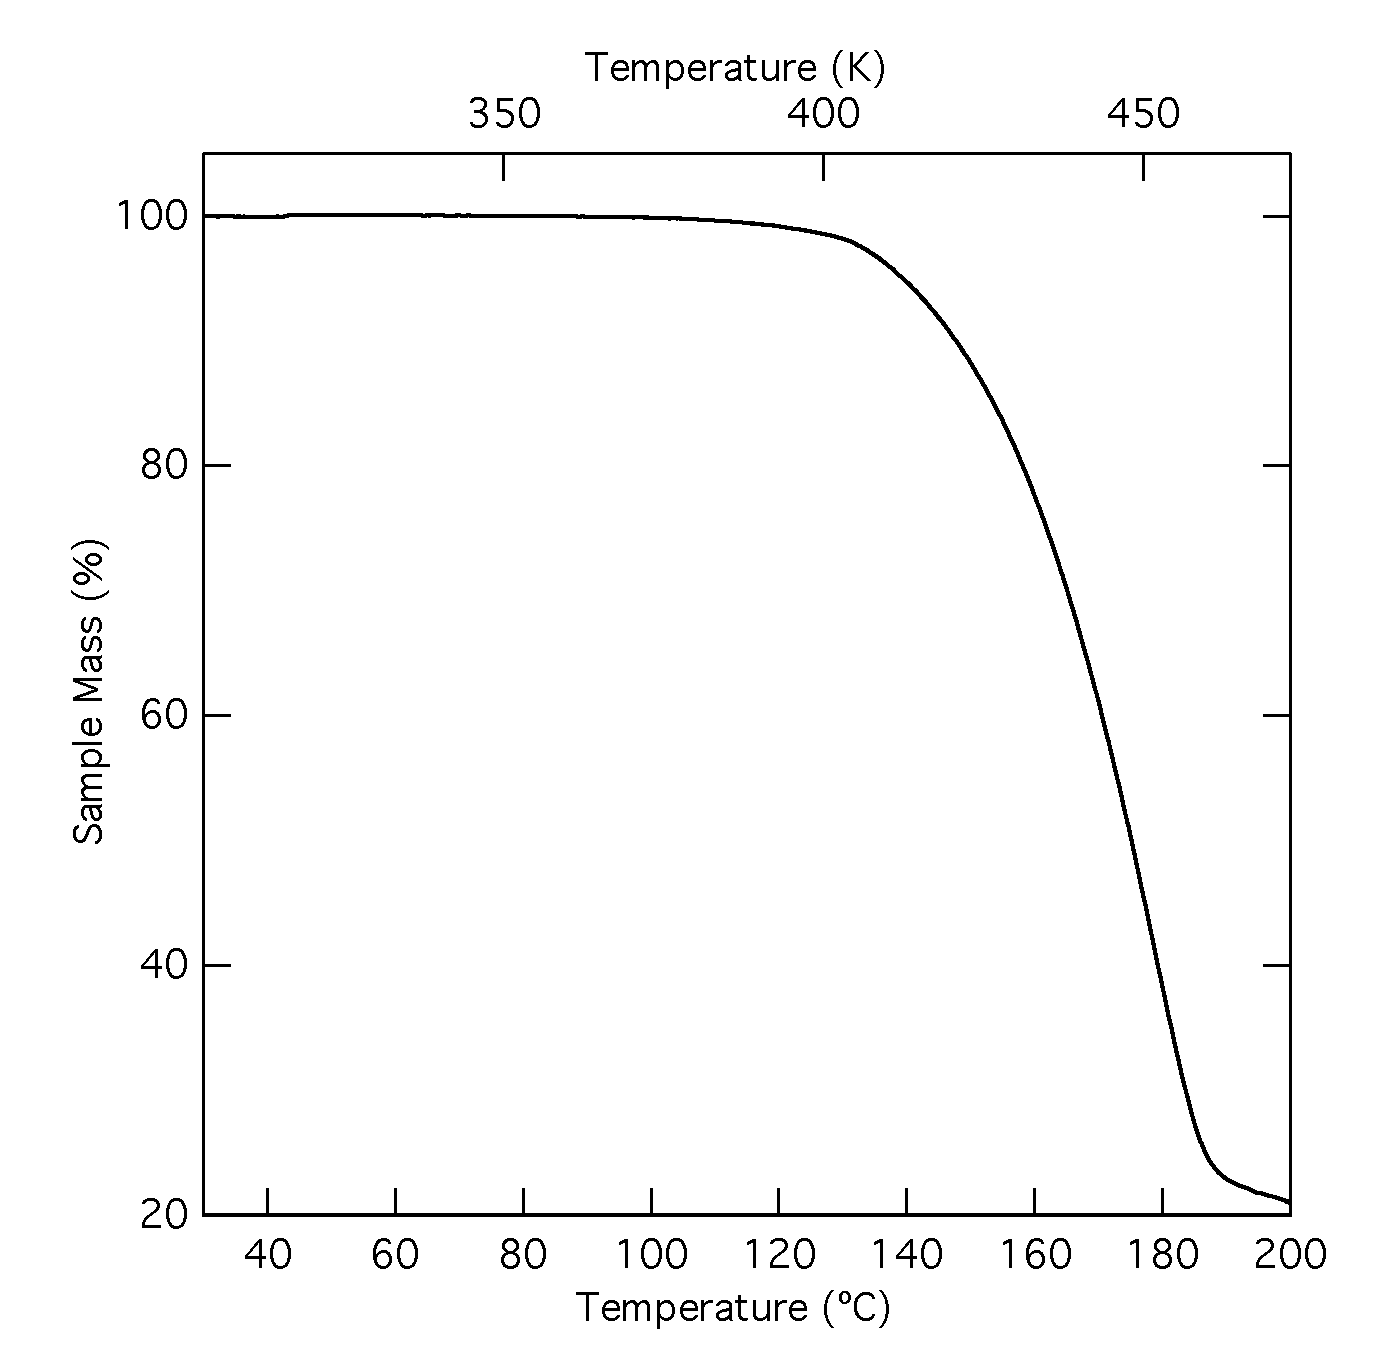
\includegraphics[width=0.75\textwidth]{./Figures/Appendix/Thermal-Analysis/TGA/TMHD-Weight}%
%%	} \\
%%%	\hspace{1cm}
%%  \subfloat[Derivative of Mass vs. Temperature][Derivative of Mass vs. Temperature]{%
%%   	\label{fig:TGA-TMHD-DWeight}%
%%	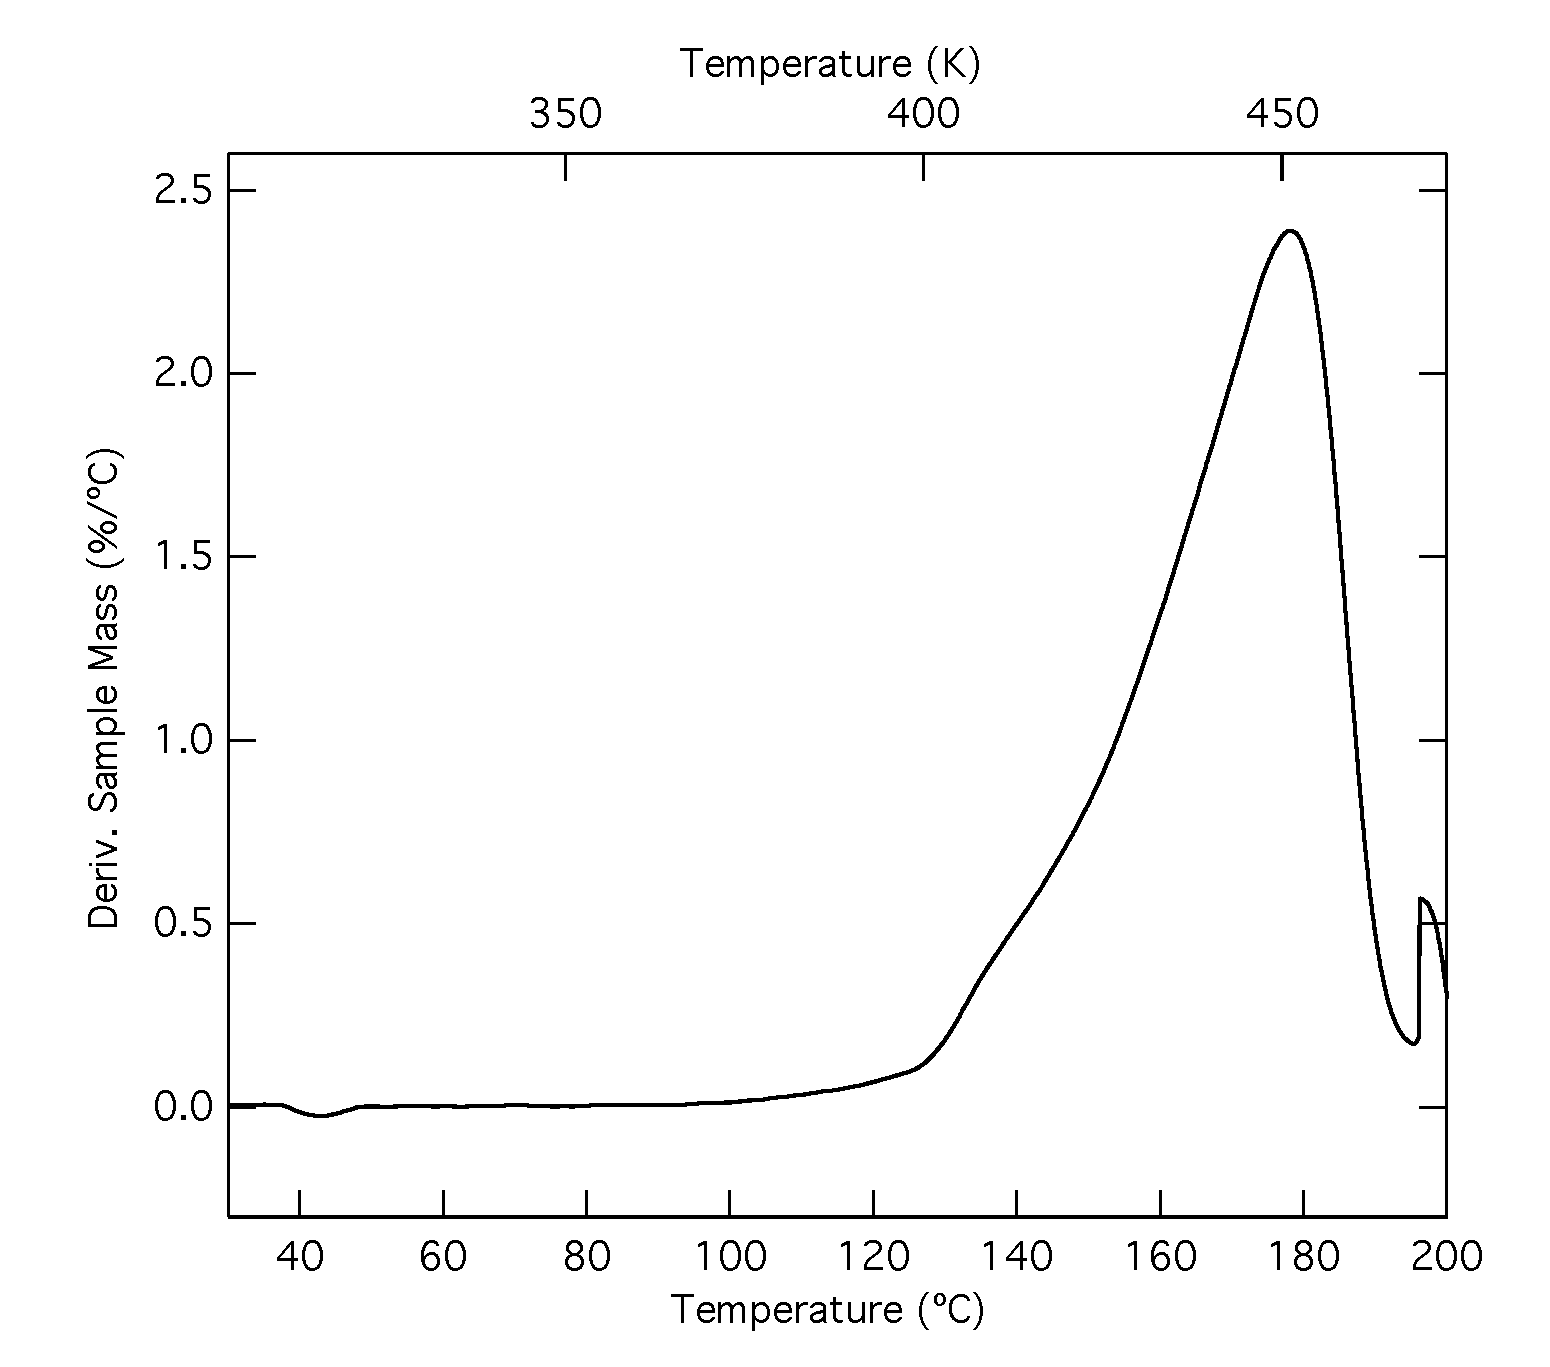
\includegraphics[width=0.75\textwidth]{./Figures/Appendix/Thermal-Analysis/TGA/TMHD-DWeight}%
%%	} 	
%%   \caption[TGA Results for Pb(HFAc)$_{2}$ Precursor]%
%%   		{Plots of the results from TGA experiments on Pb(TMHD)$_{2}$. As in figure~\vref{fig:TGA-HFAc}, (a) %
%%		presents the actual mass as a function of temperature, while (b) gives the derivative of that function. %
%%		Initial sample mass: 3.719 mg}
%%   \label{fig:TGA-TMHD}
%%\end{figure}
%
%
%%\begin{figure}[htbp]
%%   \centering
%%   \subfloat[\HFAc][\HFAc]{%
%%   	\label{fig:TGA-HFAc-Hold}%
%%	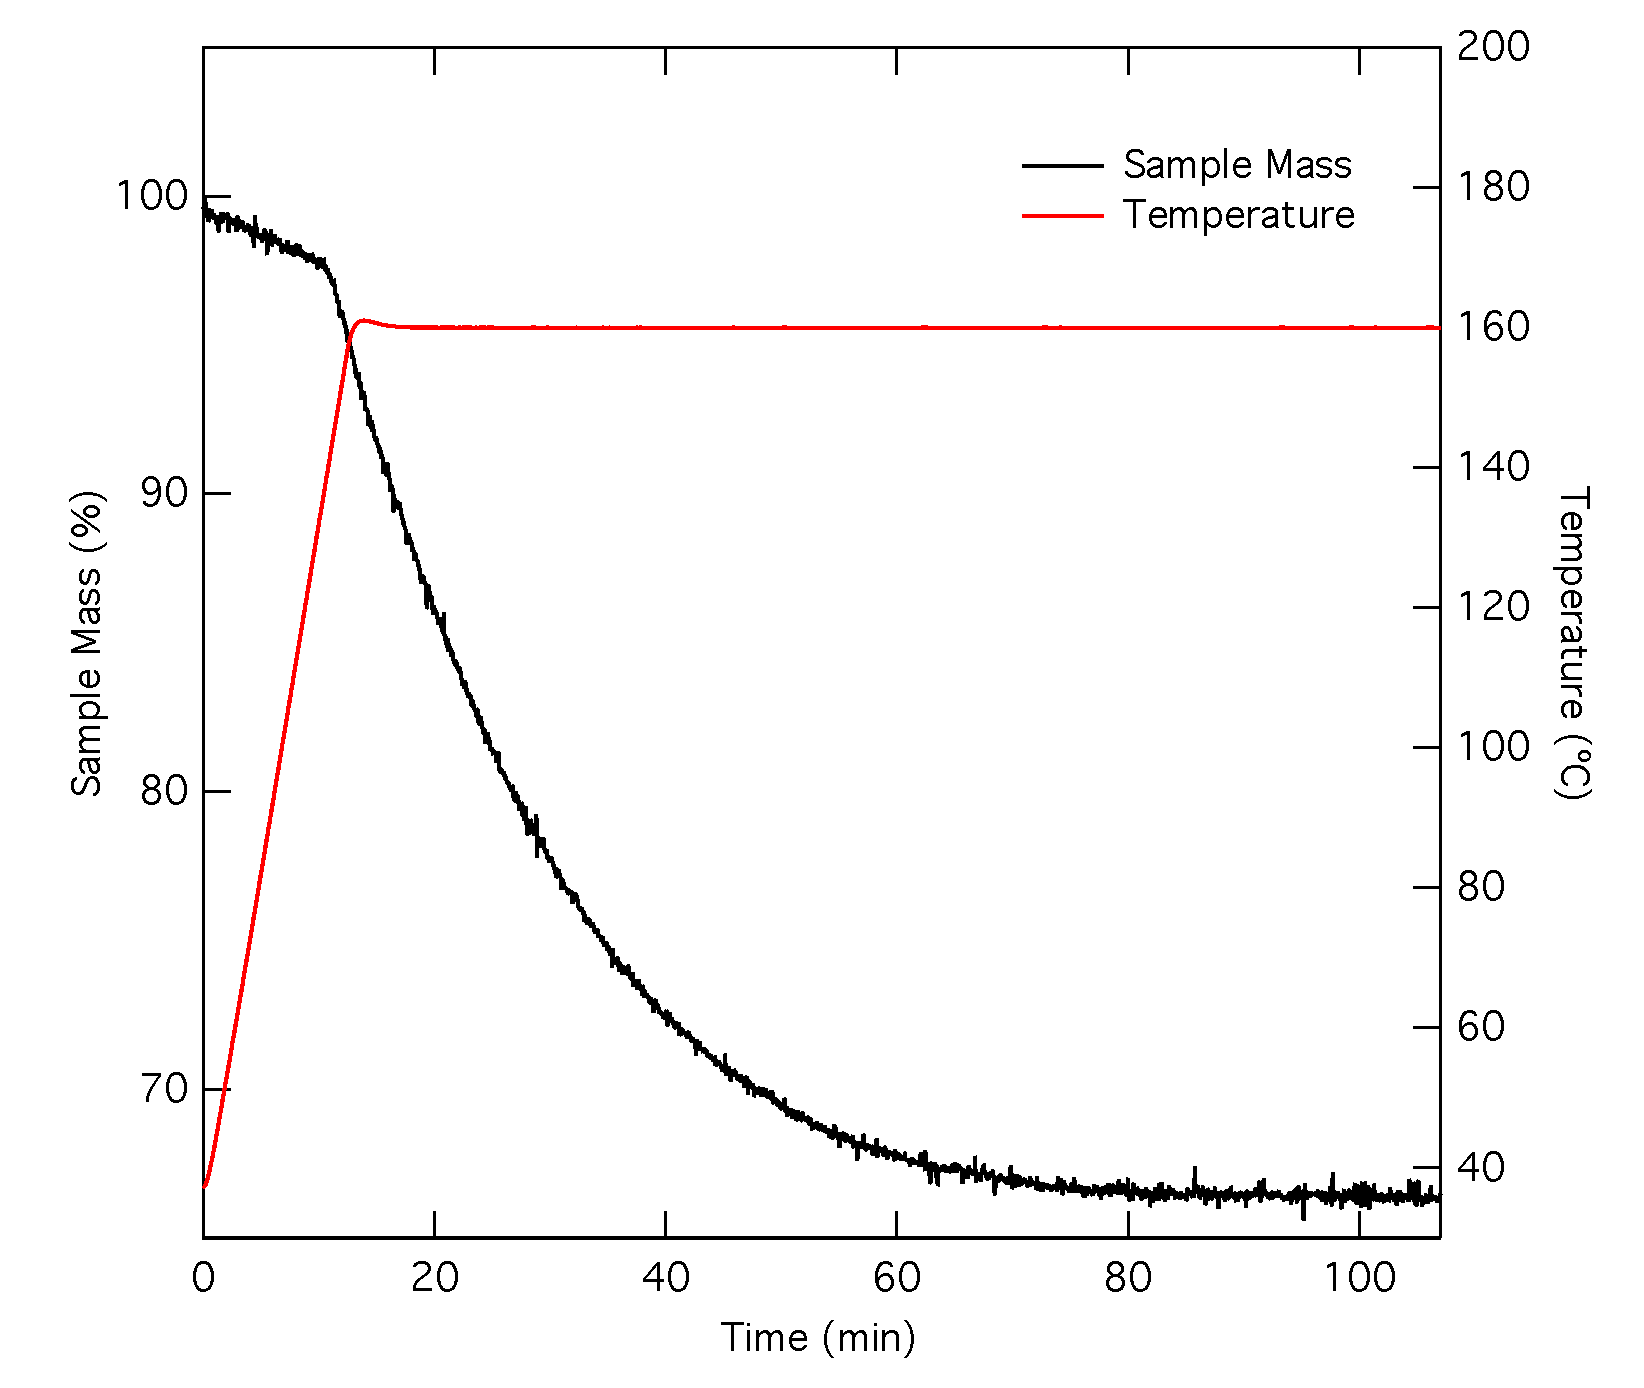
\includegraphics[width=0.75\textwidth]{./Figures/Appendix/Thermal-Analysis/TGA/HFAc-Hold}%
%%	} \\
%%%	\hspace{1cm}
%%  \subfloat[\TMHD][\TMHD]{%
%%   	\label{fig:TGA-TMHD-Hold}%
%%	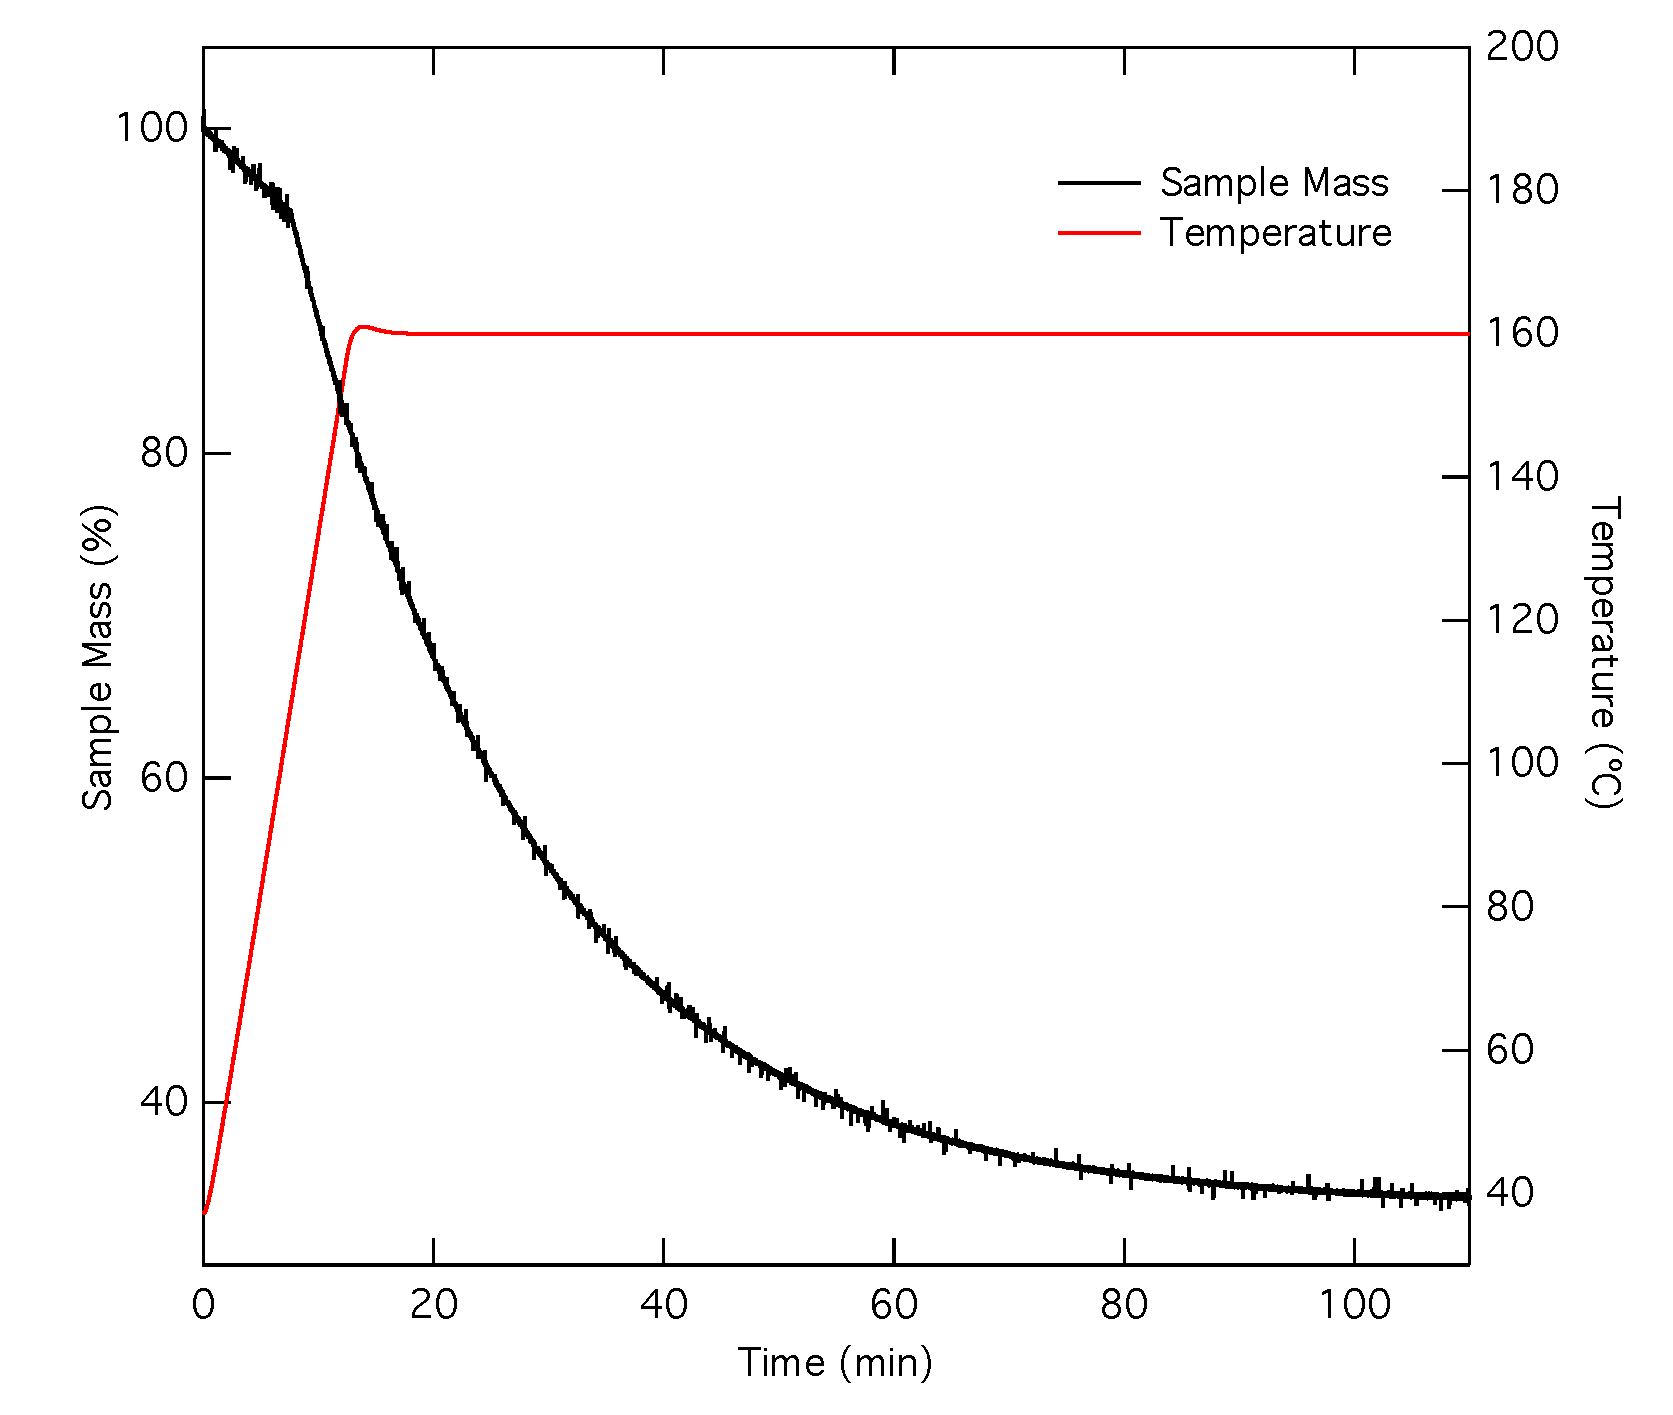
\includegraphics[width=0.75\textwidth]{./Figures/Appendix/Thermal-Analysis/TGA/TMHD-Hold}%
%%	} 	
%%   \caption[Constant Temperature TGA Experiments]%
%%   		{Plots of the results from ramp-and-hold TGA experiments designed to investigate residual material %
%%		after complete evaporation at a given temperature. From the TGA experiments seen above (figs.~%
%%		\vref{fig:TGA-HFAc} and \vref{fig:TGA-TMHD}), a common temperature of 160\degC{} was chosen %
%%		for this experiment. Sample sizes were 3.921 mg and 4.381 mg for \HFAc{} and \TMHD{} respectively.}
%%   \label{fig:TGA-Hold}
%%\end{figure}
%
%\clearpage
%
%%%%%%%%%%%%%%%%%%%%%%%%%%%%%

%\subsection{Differential Scanning Calorimetry}
%\label{sup:Thermal-Results-DSC}

%\begin{figure}[htbp]
%   \centering
%   \subfloat[Pb(HFAc)$_{2}$][Pb(HFAc)$_{2}$]{%
%   	\label{fig:DSC-HFAc}%
%	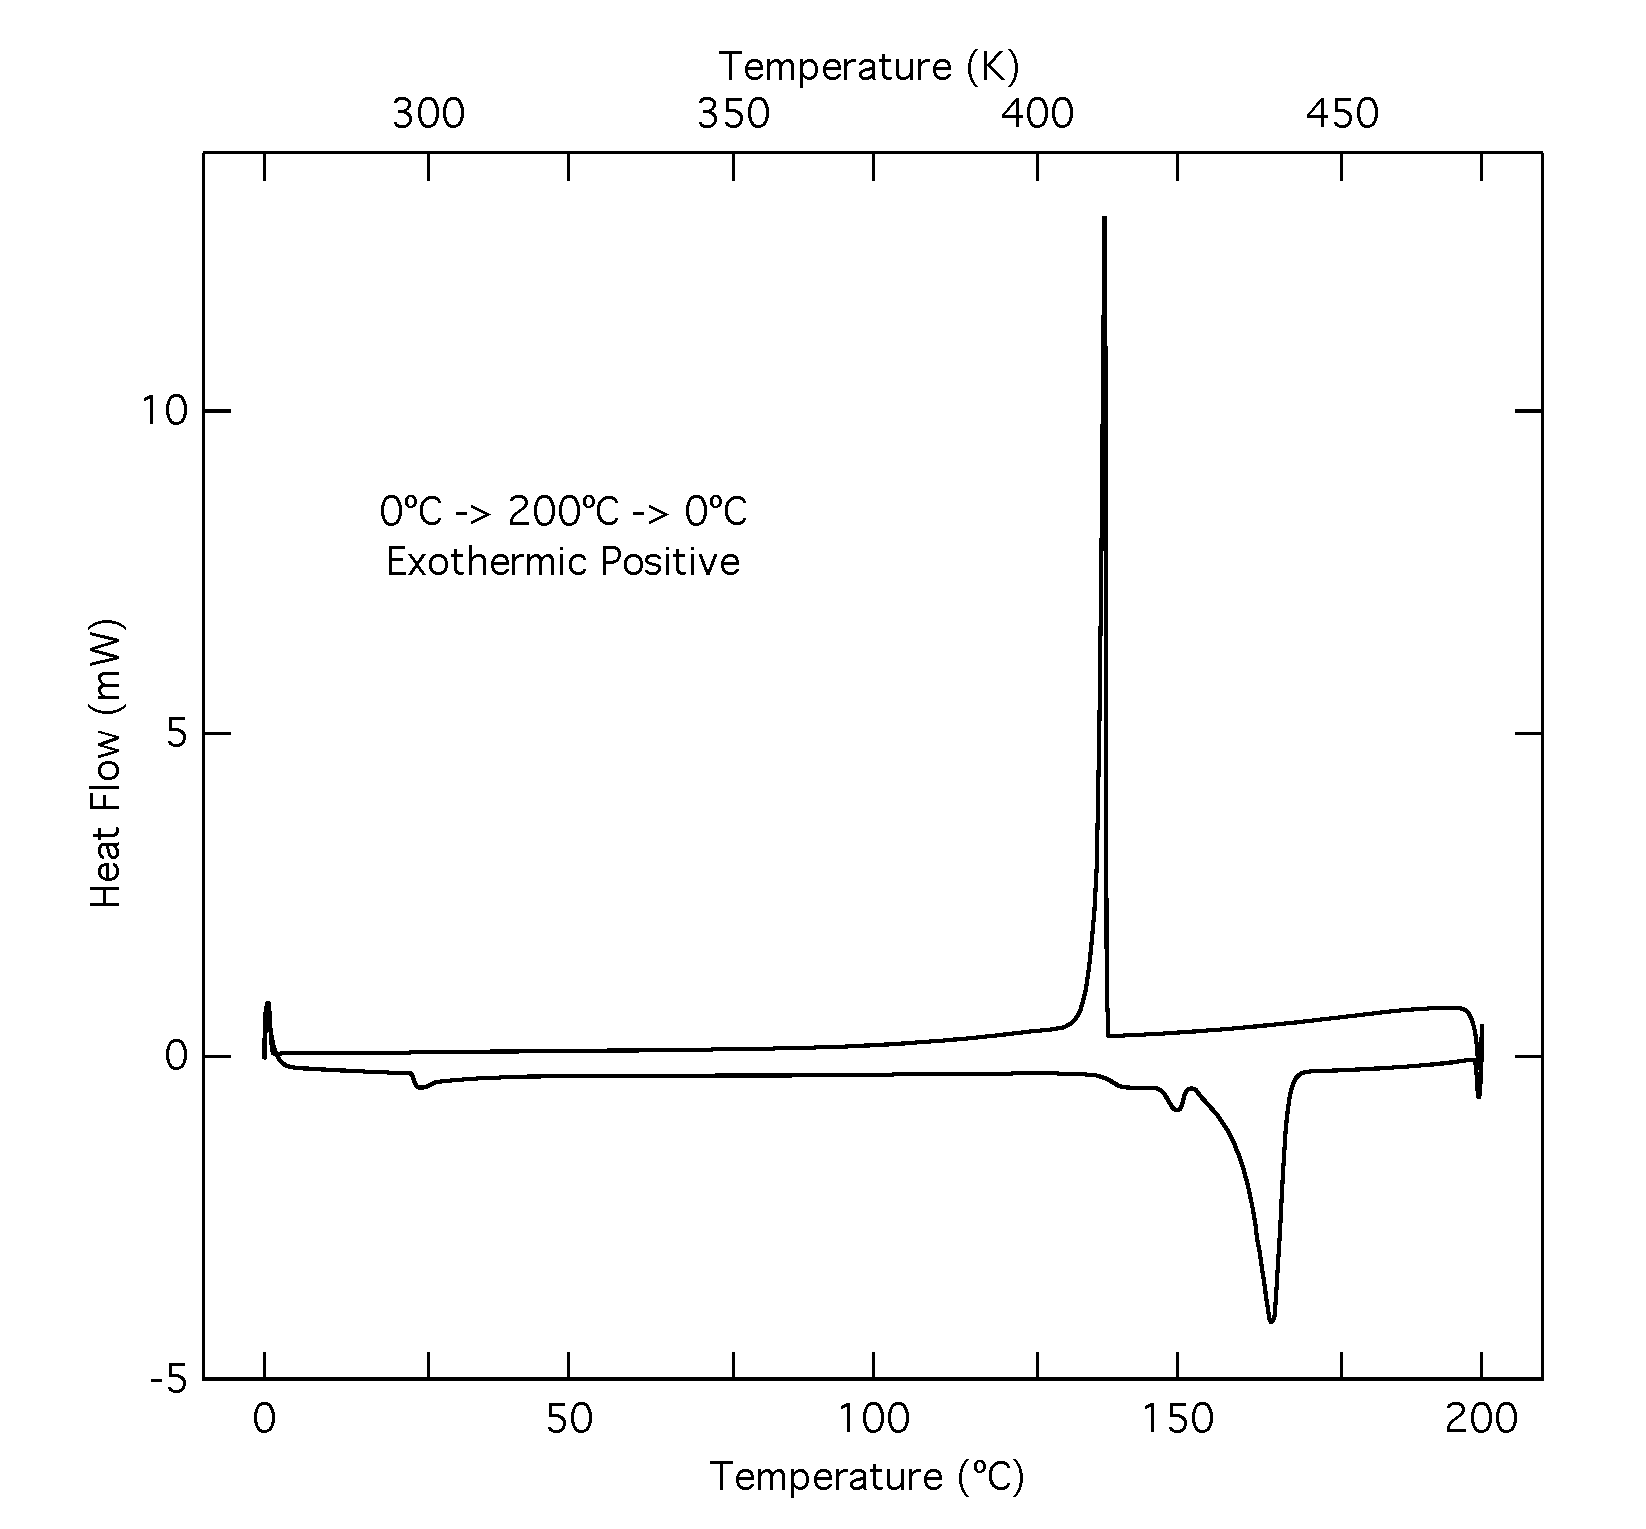
\includegraphics[width=0.75\textwidth]{./Figures/Appendix/Thermal-Analysis/DSC/HFAc}%
%	} \\
%  \subfloat[Pb(TMHD)$_{2}$][Pb(TMHD)$_{2}$]{%
%   	\label{fig:DSC-TMHD}%
%	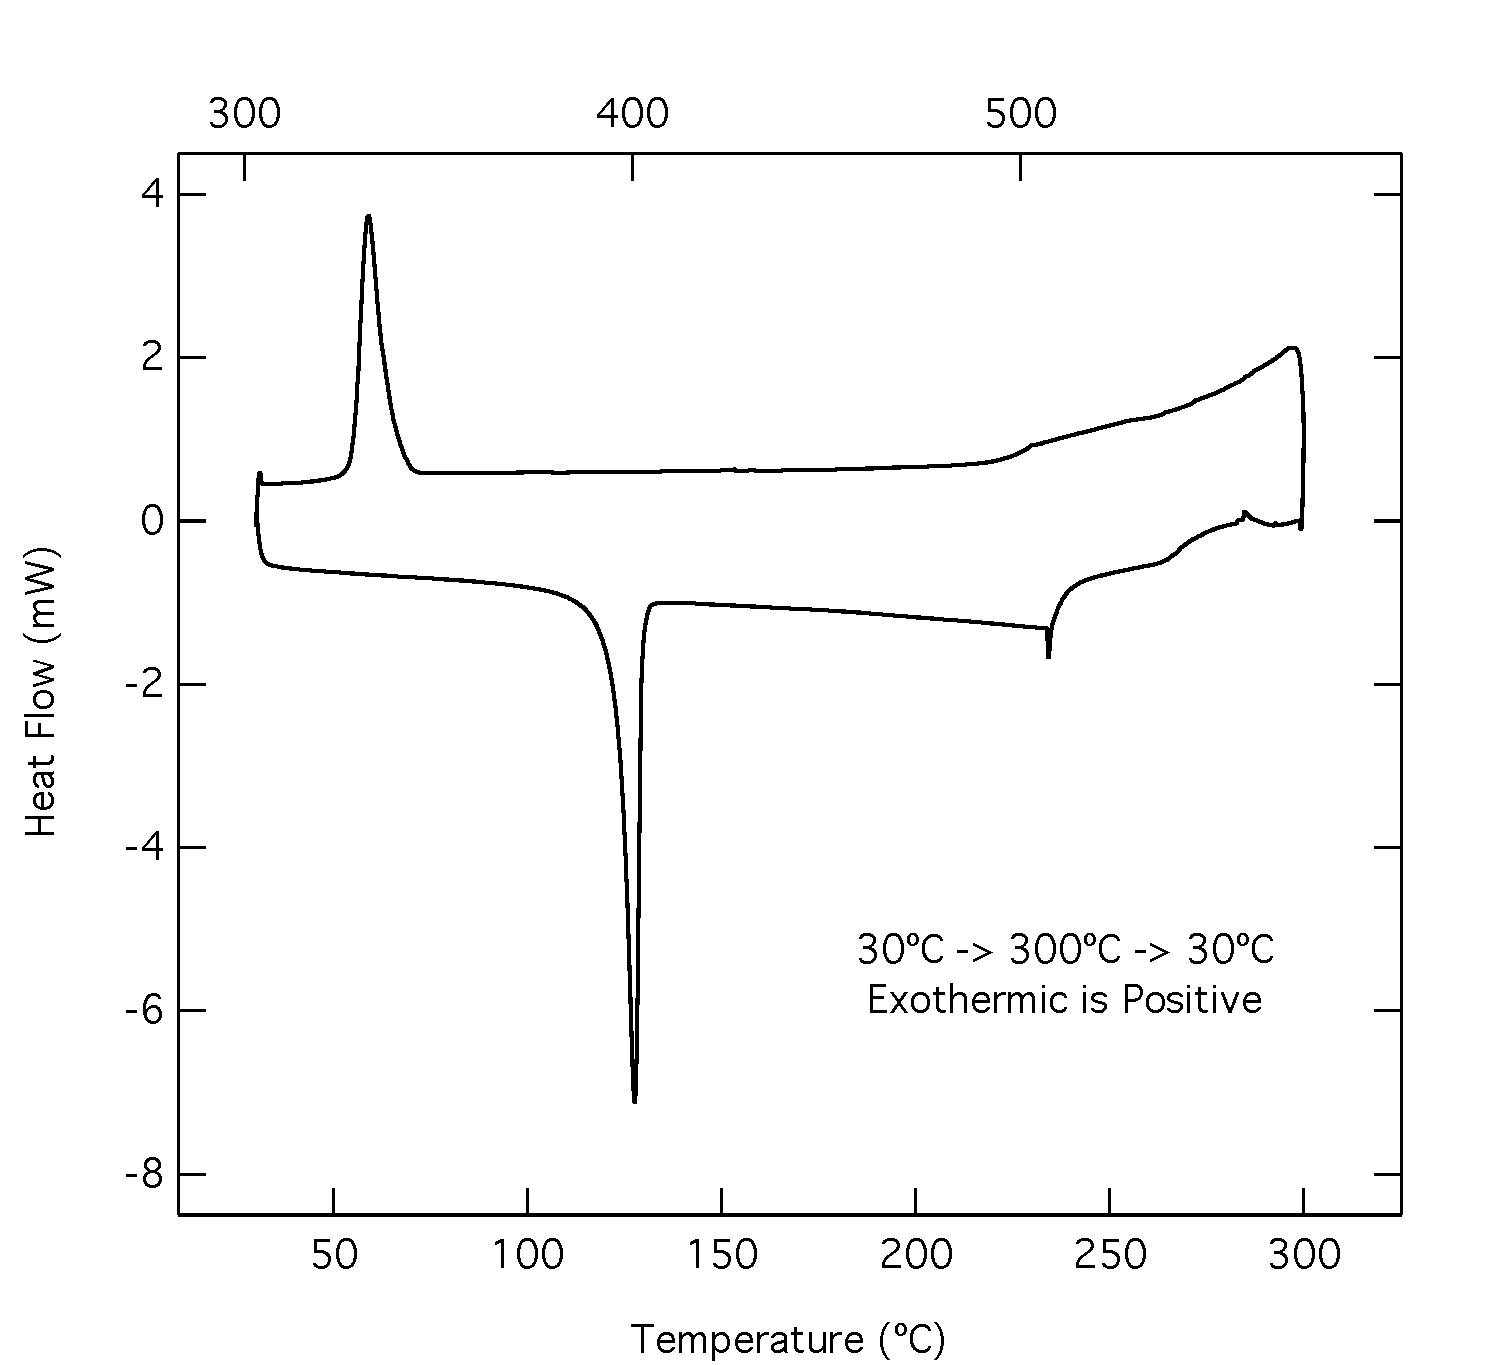
\includegraphics[width=0.75\textwidth]{./Figures/Appendix/Thermal-Analysis/DSC/TMHD}%
%	} 	
%   \caption[Results of DSC Experiments]%
%   		{This plot shows results from DSC experiments carried out during the course of %
%		this project. (a) shows the results from analyzing the Pb(HFAC)$_{2}$ compound. (b) gives %
%		the data from Pb(TMHD)$_{2}$. Exothermic (heat release) flow is positive in both plots. }
%   \label{fig:DSC-Data}
%\end{figure}

%\clearpage

%\begin{figure}[htbp]
%	\begin{center}
%		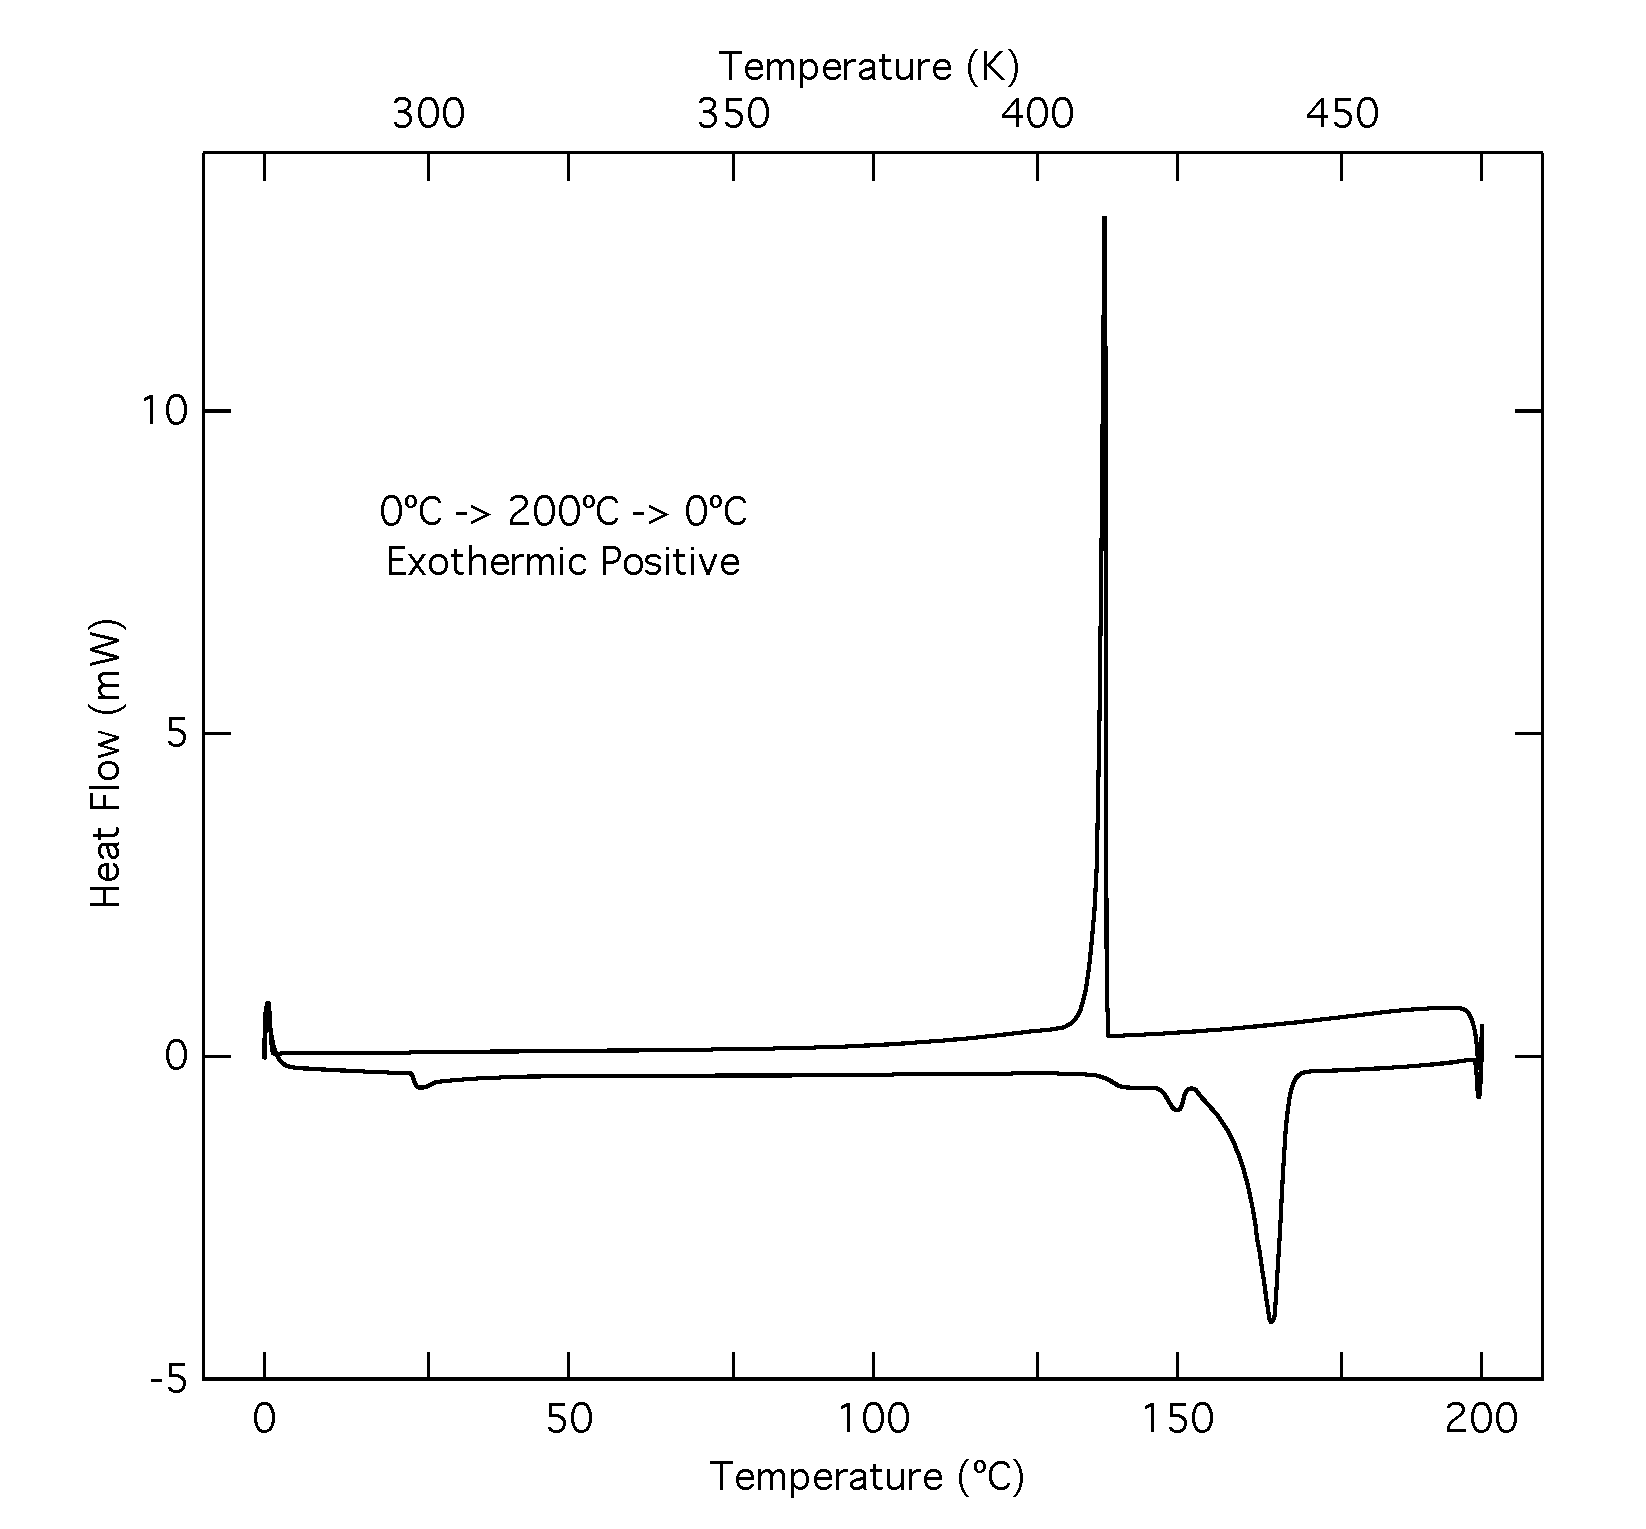
\includegraphics[width=0.75\textwidth]{./Figures/Appendix/Thermal-Analysis/DSC/HFAc}
%		\caption[DSC of Pb(HFAc)$_{2}$]{This plot shows the result of a DSC experiment on the %
%				Pb(HFAc)$_{2}$ precursor. It shows the major points where energy is absorbed or %
%				released, and analysis of these points can give significant information about the %
%				thermal behavior and the transition mechanisms.}
%		\label{fig:DSC-HFAc}
%	\end{center}
%\end{figure}
%
%\begin{figure}[htbp]
%	\begin{center}
%		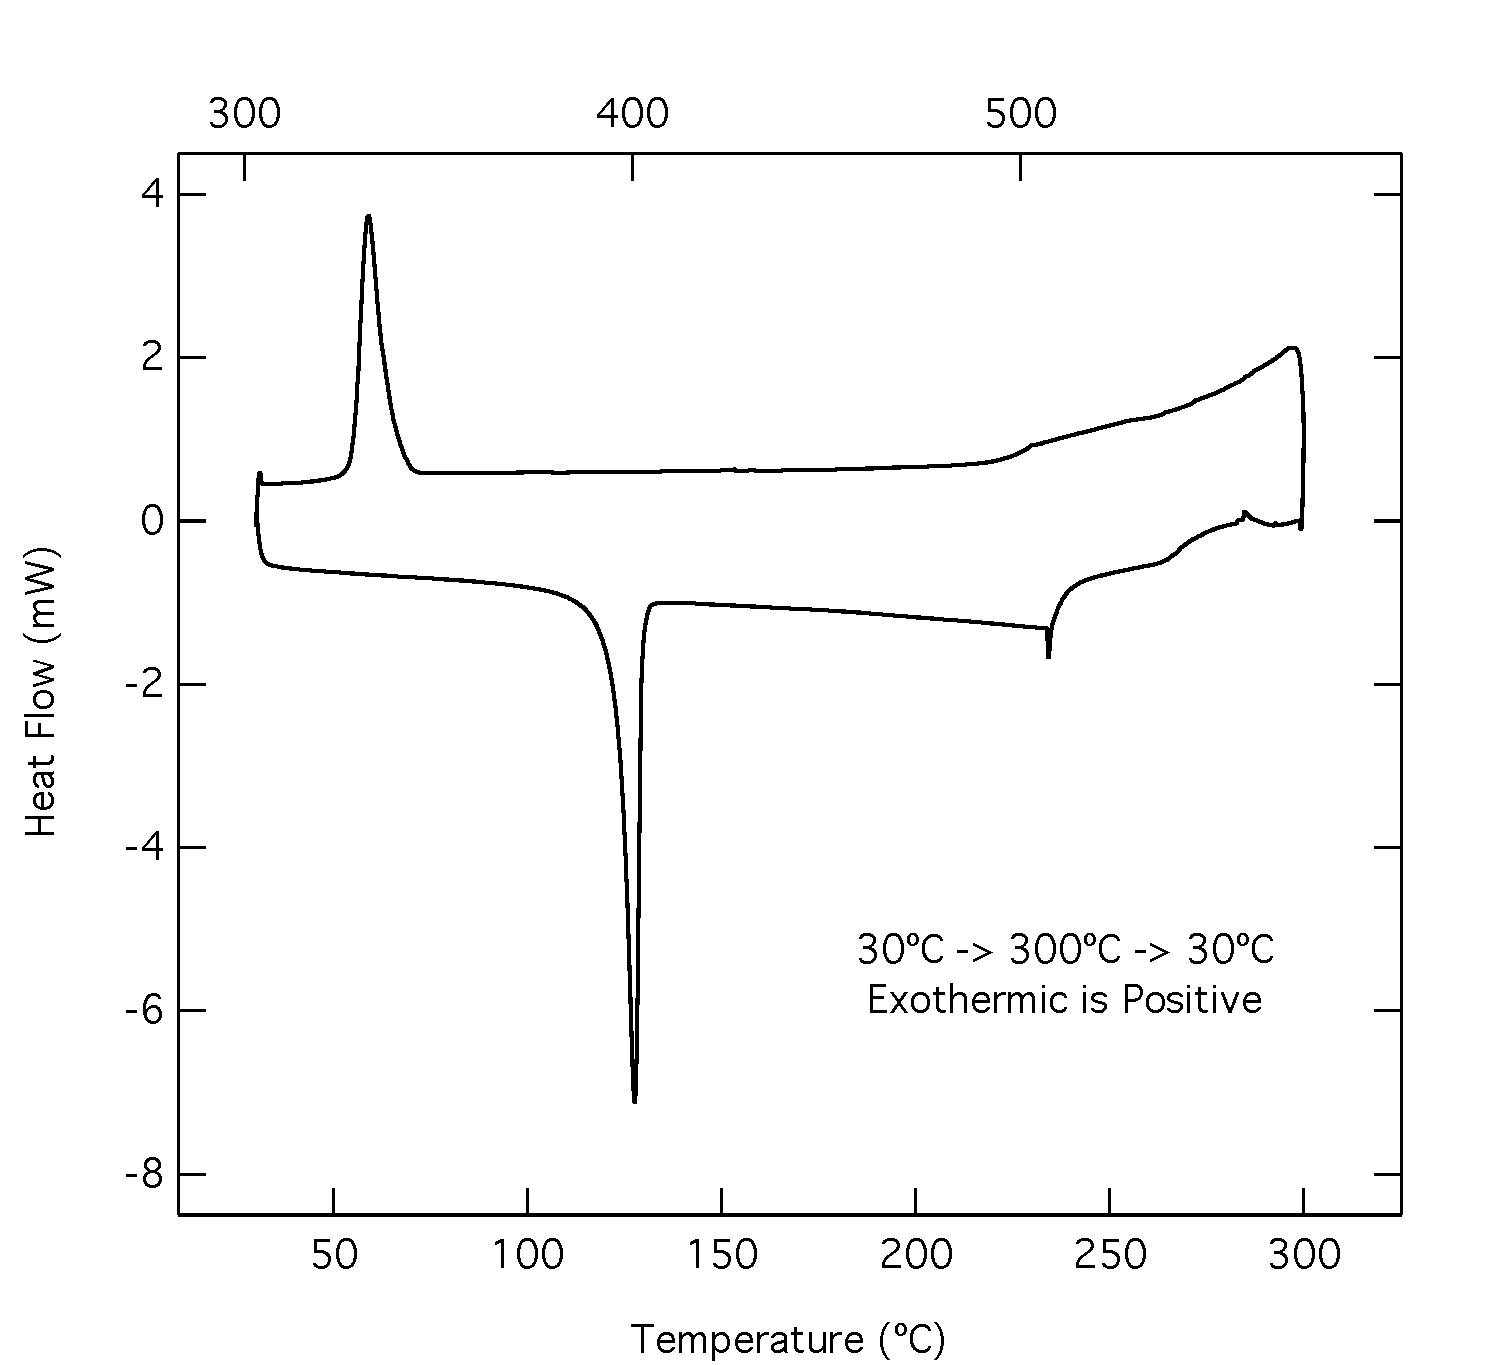
\includegraphics[width=0.75\textwidth]{./Figures/Appendix/Thermal-Analysis/DSC/TMHD}
%		\caption[DSC of Pb(TMHD)$_{2}$]{This plot shows the result of a DSC experiment on the %
%				Pb(TMHD)$_{2}$ precursor. As in figure~\vref{fig:DSC-HFAc}, analysis of this plot %
%				can give meaningful information on what is chemically happening to the %
%				compound as the temperature changes.}
%		\label{fig:DSC-TMHD}
%	\end{center}
%\end{figure}

%%%%%%%%%%%%%%%%%%%%%%%%%%%%%%%%%%%%%%%%%%%%%%%%%%%%
%%%%%%%%%%%%%%%%%%%%%%%%%%%%%%%%%%%%%%%%%%%%%%%%%%%%
%%%%%%%%%%%%%%%%%%%%%%%%%%%%%%%%%%%%%%%%%%%%%%%%%%%%

\section{Composition Results}
\label{sup:Composition}

%\begin{table}[htbp]
%	\centering
%	\caption[XRF Calculated Compositions]{Calculated compositions of selected samples, determined via XRF. \\Composition percentages are all $\pm$1\%.\label{tbl:XRF-compositions}}
%	\begin{tabular}{l l r r r}
%	\toprule
%	&&\multicolumn{3}{c}{Composition (\%)}\\
%	\cmidrule{3-5}
%	Run \#&Substrate&Lead&Titanium&Ti:Pb Ratio\\
%	\midrule
%% 	Run	Sub-Type		Pb%		Ti%		Ti:Pb ratio
%	0	&\ce{SiO2}	&55.99	&44.01	&0.786\\
%	1	&\ce{SiO2}	&55.00	&45.00	&0.809\\
%	13	&\ce{SiO2}	&53.96	&46.04	&0.853\\
%	16	&\ce{SiO2}	&49.45	&50.55	&1.022\\
%	19	&\ce{SiO2}	&65.87	&34.13	&0.518\\
%		&Pt-Si		&42.86	&57.14	&1.333\\
%	20	&\ce{SiO2}	&56.52	&43.48	&0.769\\
%		&\ce{Pt-Si}	&51.43	&48.57	&0.944\\
%	21	&\ce{SiO2}	&69.60	&30.40	&0.437\\
%		&Pt-Si		&56.08	&43.92	&0.783\\
%	22	&\ce{SiO2}	&67.64	&32.36	&0.478\\
%		&Pt-Si		&56.06	&43.94	&0.784\\
%	23	&\ce{SiO2}	&66.89	&33.11	&0.495\\
%		&Pt-Si		&49.06	&50.94	&1.038\\
%	24	&\ce{SiO2}	&68.96	&31.06	&0.450\\
%		&Pt-Si		&62.16	&37.84	&0.609\\
%	\bottomrule
%	\end{tabular}
%\end{table}

\begin{figure}[htbp]
	\centering
	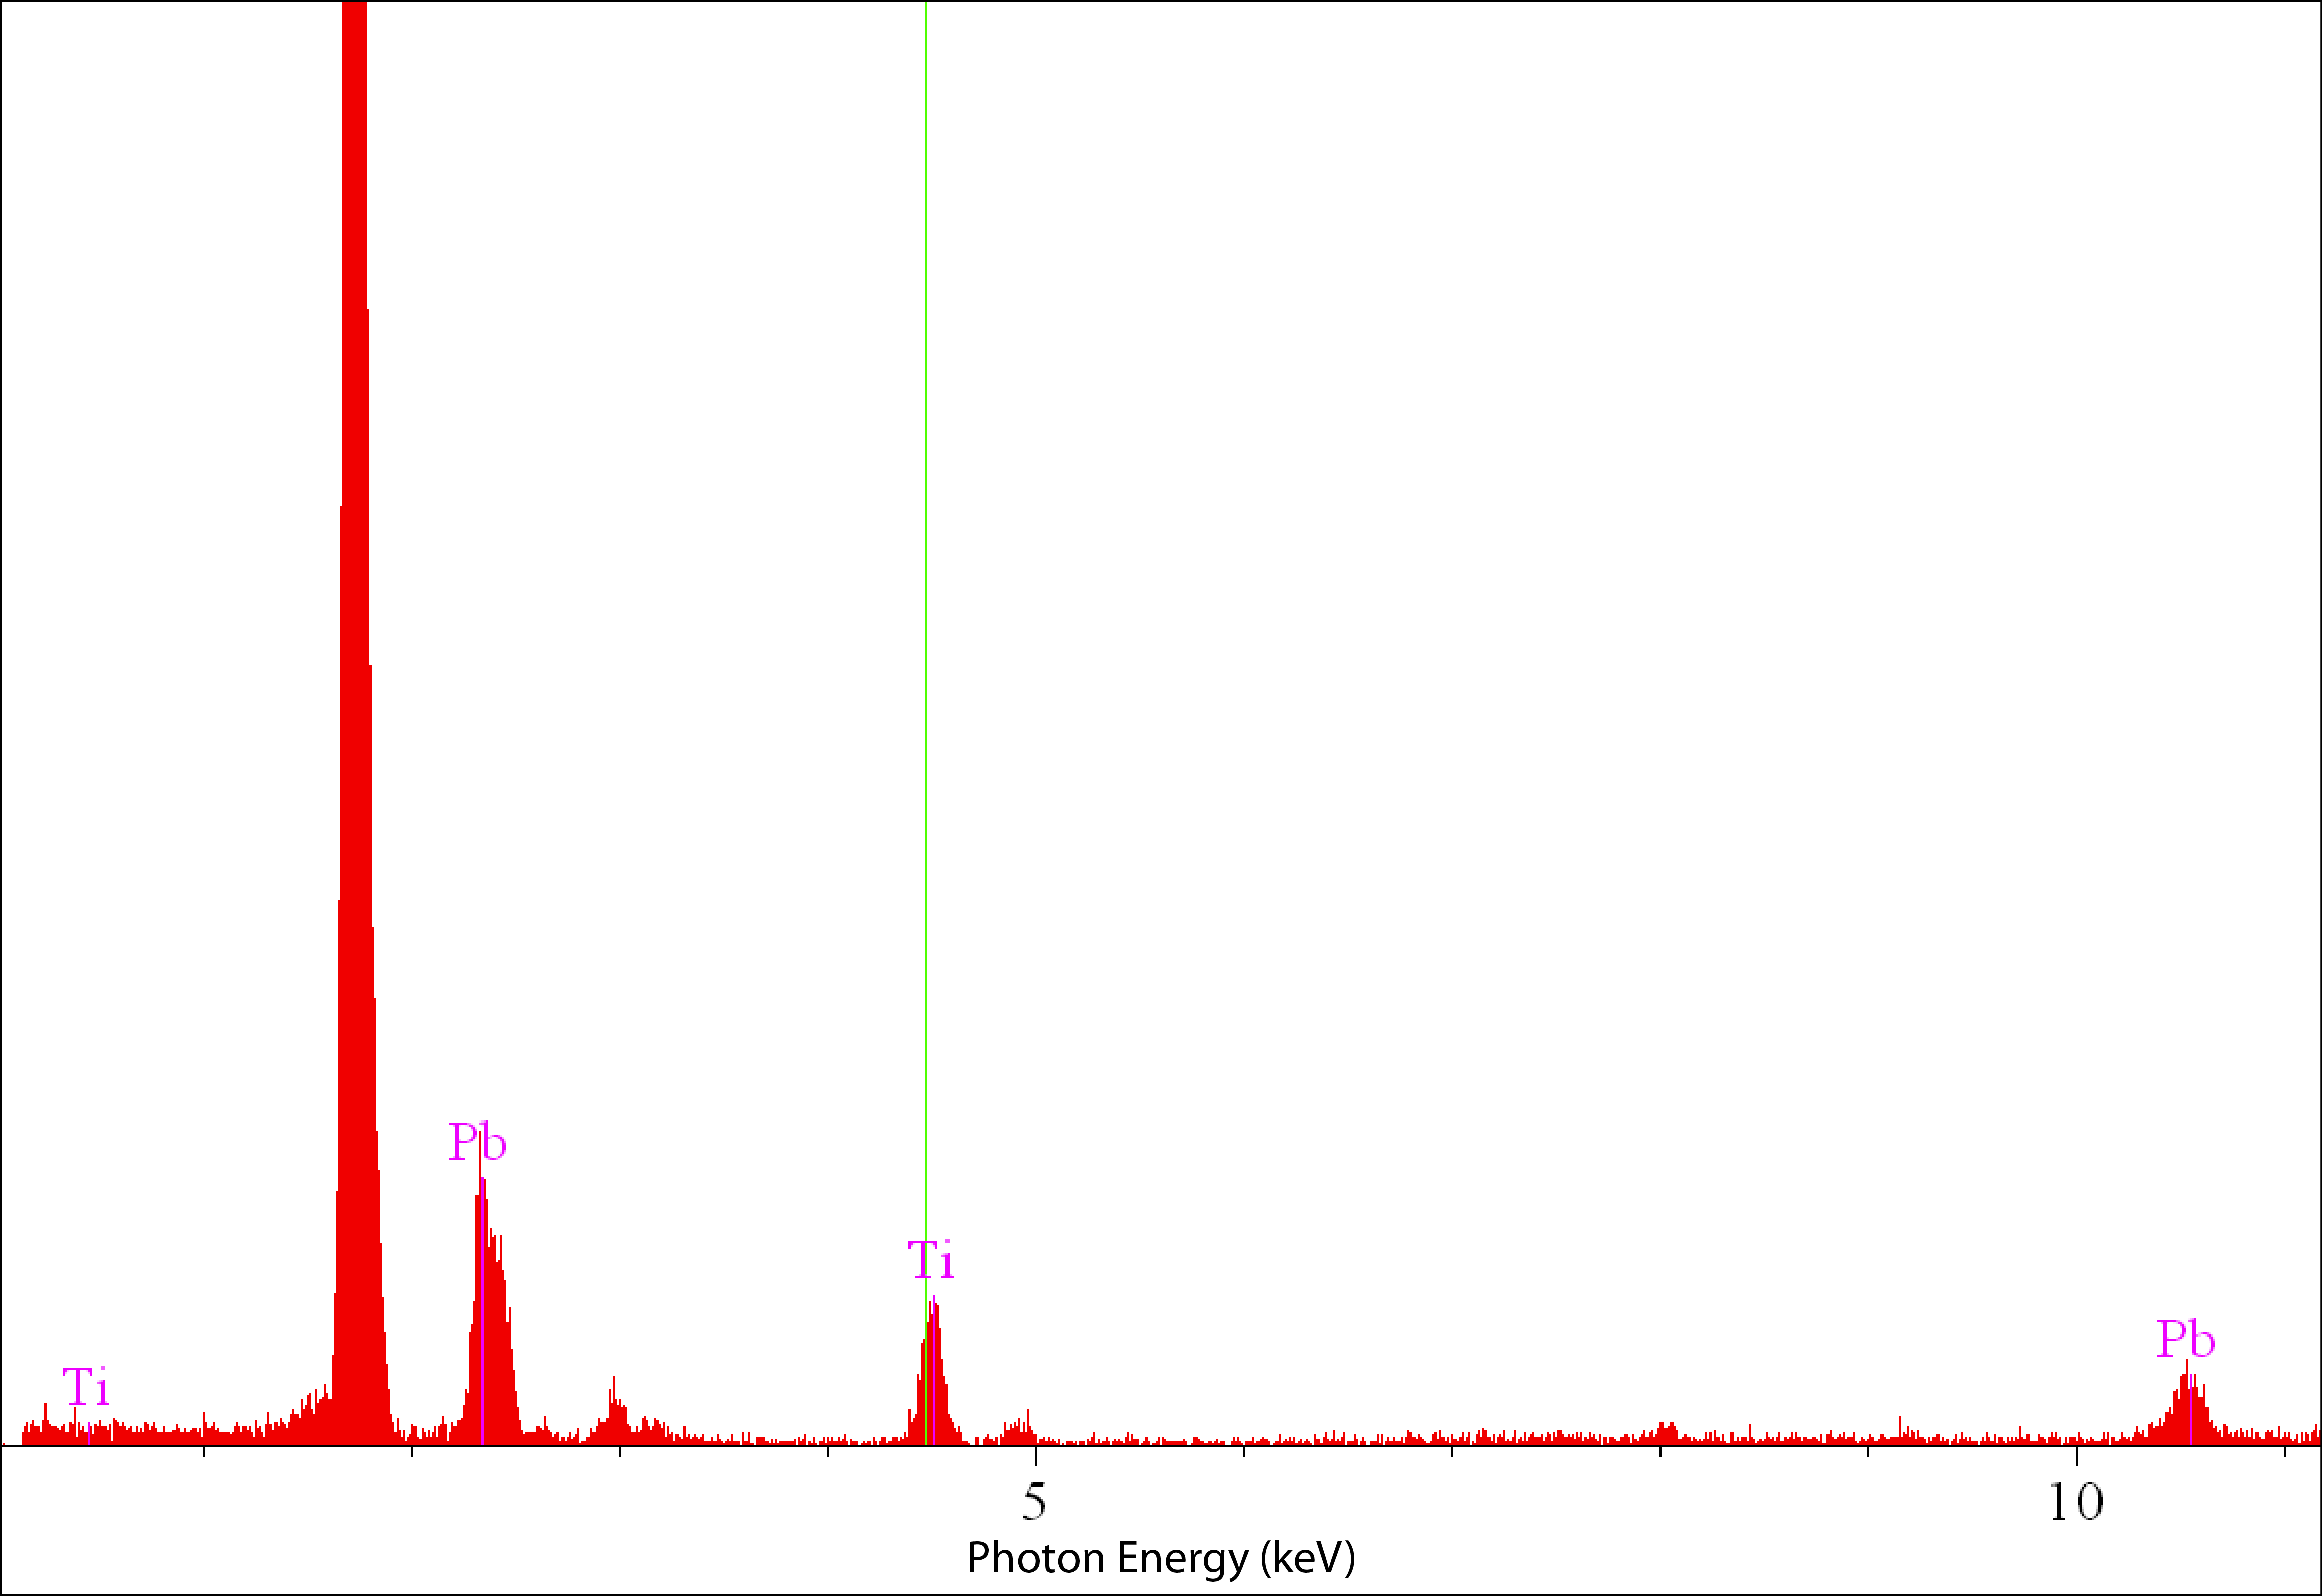
\includegraphics[width=0.85\textwidth]{./Figures/Appendix/Composition/PTO-run0-pre-anneal.png}
	\caption[XRF Spectrum of PTO \#0]%
		     {The XRF spectrum collected from deposition run \#0.  }
	\label{fig:XRF-0-SiO2}
\end{figure}

\begin{figure}[htbp]
	\centering
	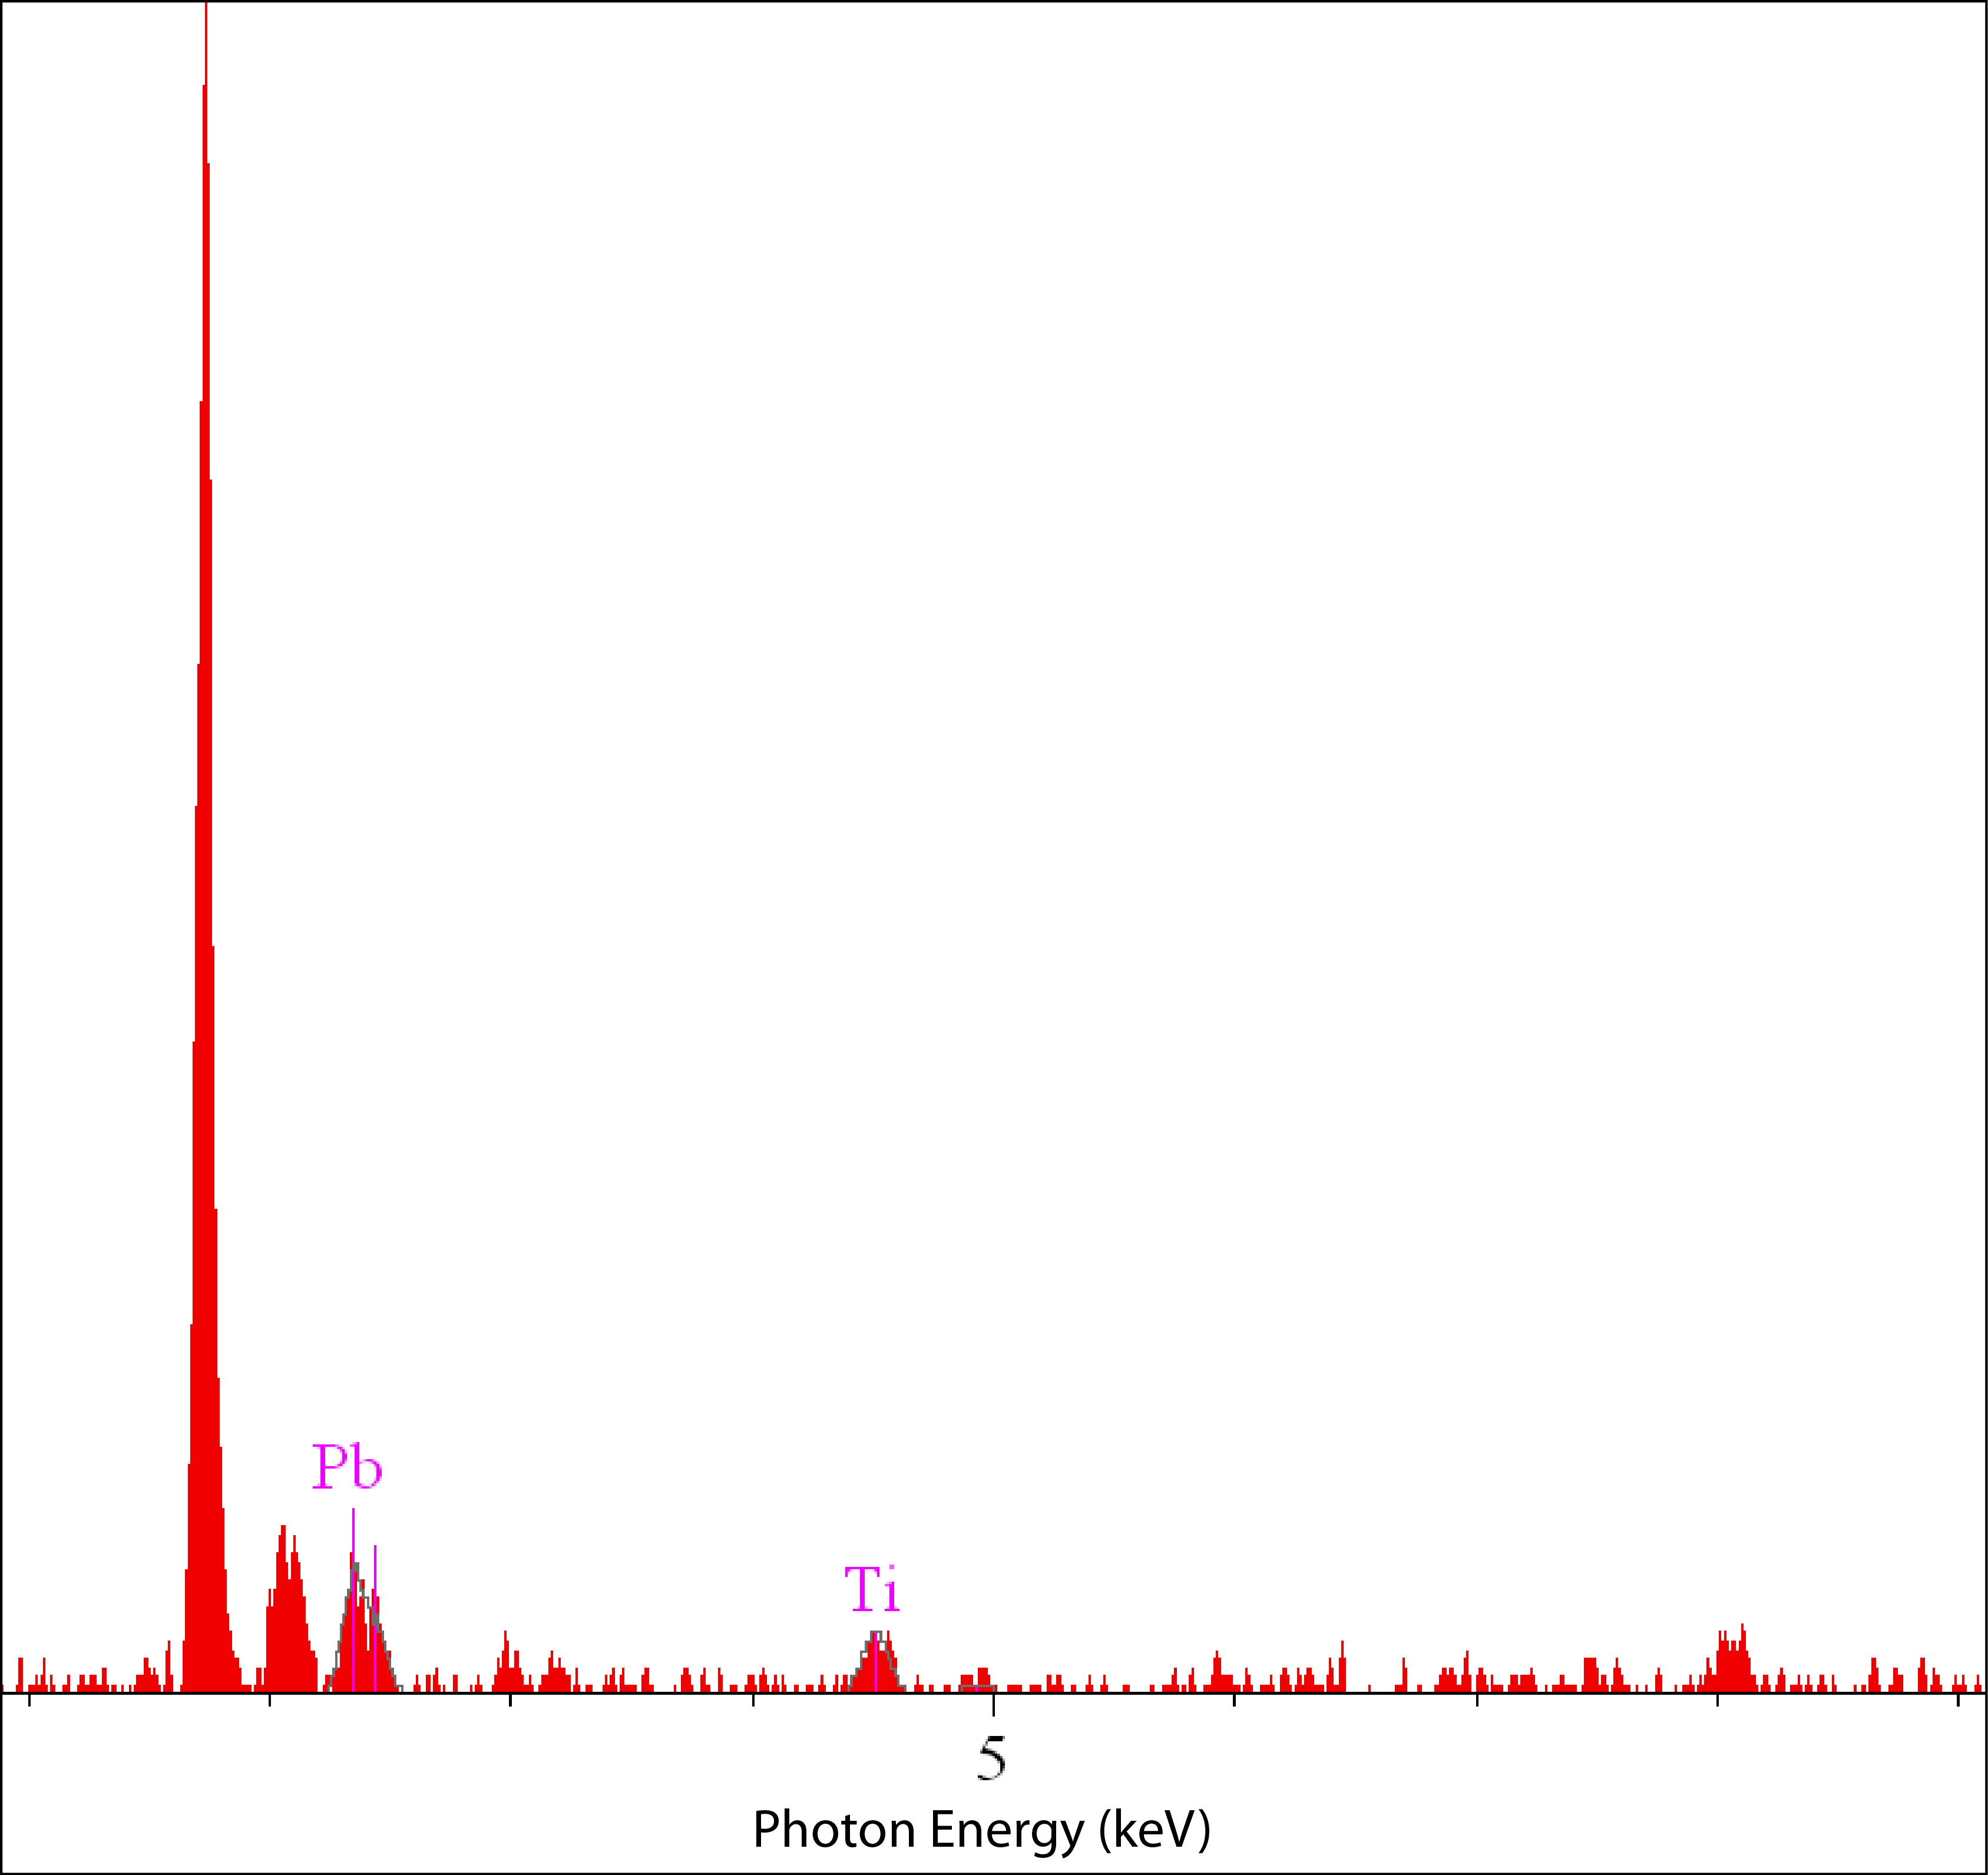
\includegraphics[width=0.85\textwidth]{./Figures/Appendix/Composition/PTO-run20-pt.png}
	\caption[XRF Spectrum of PTO \#20 on Pt-Si]%
		     {The XRF spectrum collected from deposition run \#20 deposited on platinized silicon. The peak between the substrate and Pb is that of Pt. }
	\label{fig:XRF-20-Pt}
\end{figure}

\clearpage
%%%%%%%%%%%%%%%%%%%%%%%%%%%%%%%%%%%%%%%%%%%%%%%%%%%%
%%%%%%%%%%%%%%%%%%%%%%%%%%%%%%%%%%%%%%%%%%%%%%%%%%%%
%%%%%%%%%%%%%%%%%%%%%%%%%%%%%%%%%%%%%%%%%%%%%%%%%%%%

\section{Ellipsometry Results}
\label{sup:Ellipsometry}

\begin{table}[htbp]
	\centering
	\caption[PTO \#0 Ellipsometric Model Variables]{Variables used to produce the\\model fit for PTO \#0 seen in fig.~\vref{fig:Ellip-0-SiO2}. \label{tbl:PTO-0-ellip-variables}}
	\begin{tabular}{l l r r}
	\toprule
	Layer&Variable&Thickness (nm)&Value\\
	\midrule
	2. T-L Osc.&&88.7&\\
	&$\epsilon_{1}$ offset&&2.49\\
	&Amp&&12.66\\
	&E$_{\mathrm{n}}$&&4.60\\
	&C&&1.35\\
	&E$_{\mathrm{g}}$&&0.86\\
	1. \ce{SiO2}&&203.7&\\
	0. \ce{Si}&&Substrate&\\
	\bottomrule
	\end{tabular}
\end{table}

\begin{figure}[htbp]
   \centering
   \subfloat[Psi vs. Wavelength][Psi ($\Psi$) vs. Wavelength ($\lambda$)]{%
   	\label{fig:Ellip-0-SiO2-Psi}%
	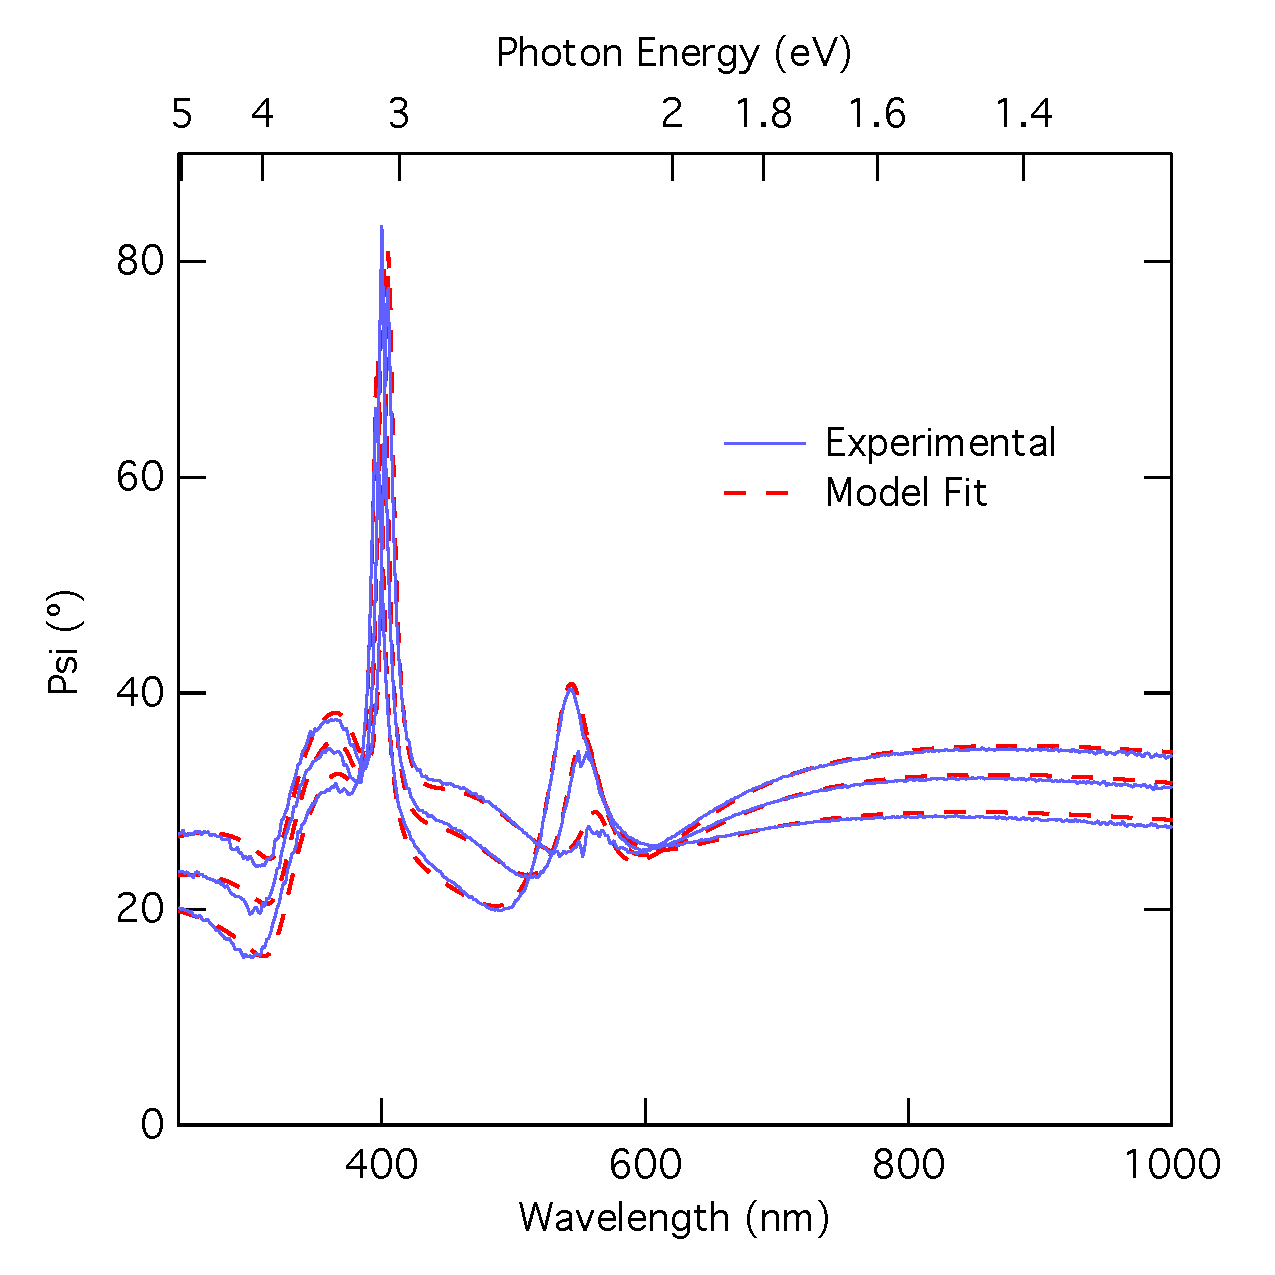
\includegraphics[width=0.47\textwidth]{./Figures/Appendix/Ellipsometry/Run-0-SiO2/Psi.pdf}%
	}\hspace{0.5cm}
  \subfloat[Delta vs. Wavelength][Delta ($\Delta$) vs. Wavelength ($\lambda$)]{%
   	\label{fig:Ellip-0-SiO2-Delta}%
	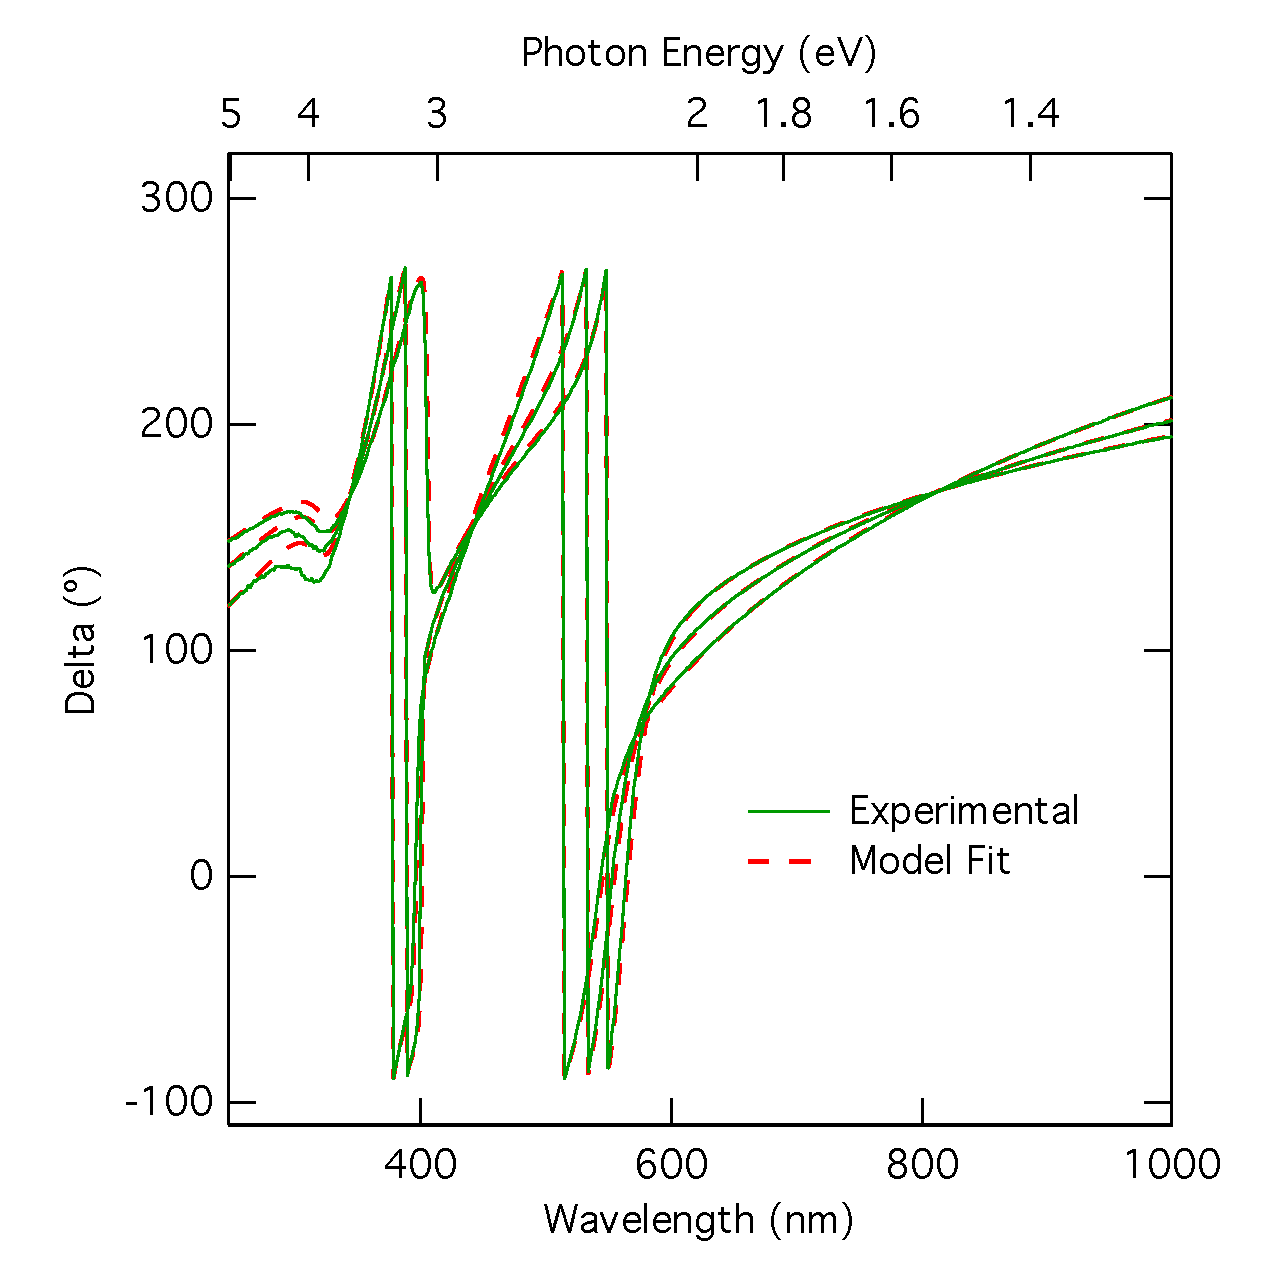
\includegraphics[width=0.47\textwidth]{./Figures/Appendix/Ellipsometry/Run-0-SiO2/Delta.pdf}%
	} \\
  \subfloat[$n$, $k$ vs. Photon Energy][$n$, $k$ vs. Photon Energy (eV)]{%
   	\label{fig:Ellip-0-SiO2-nk}%
	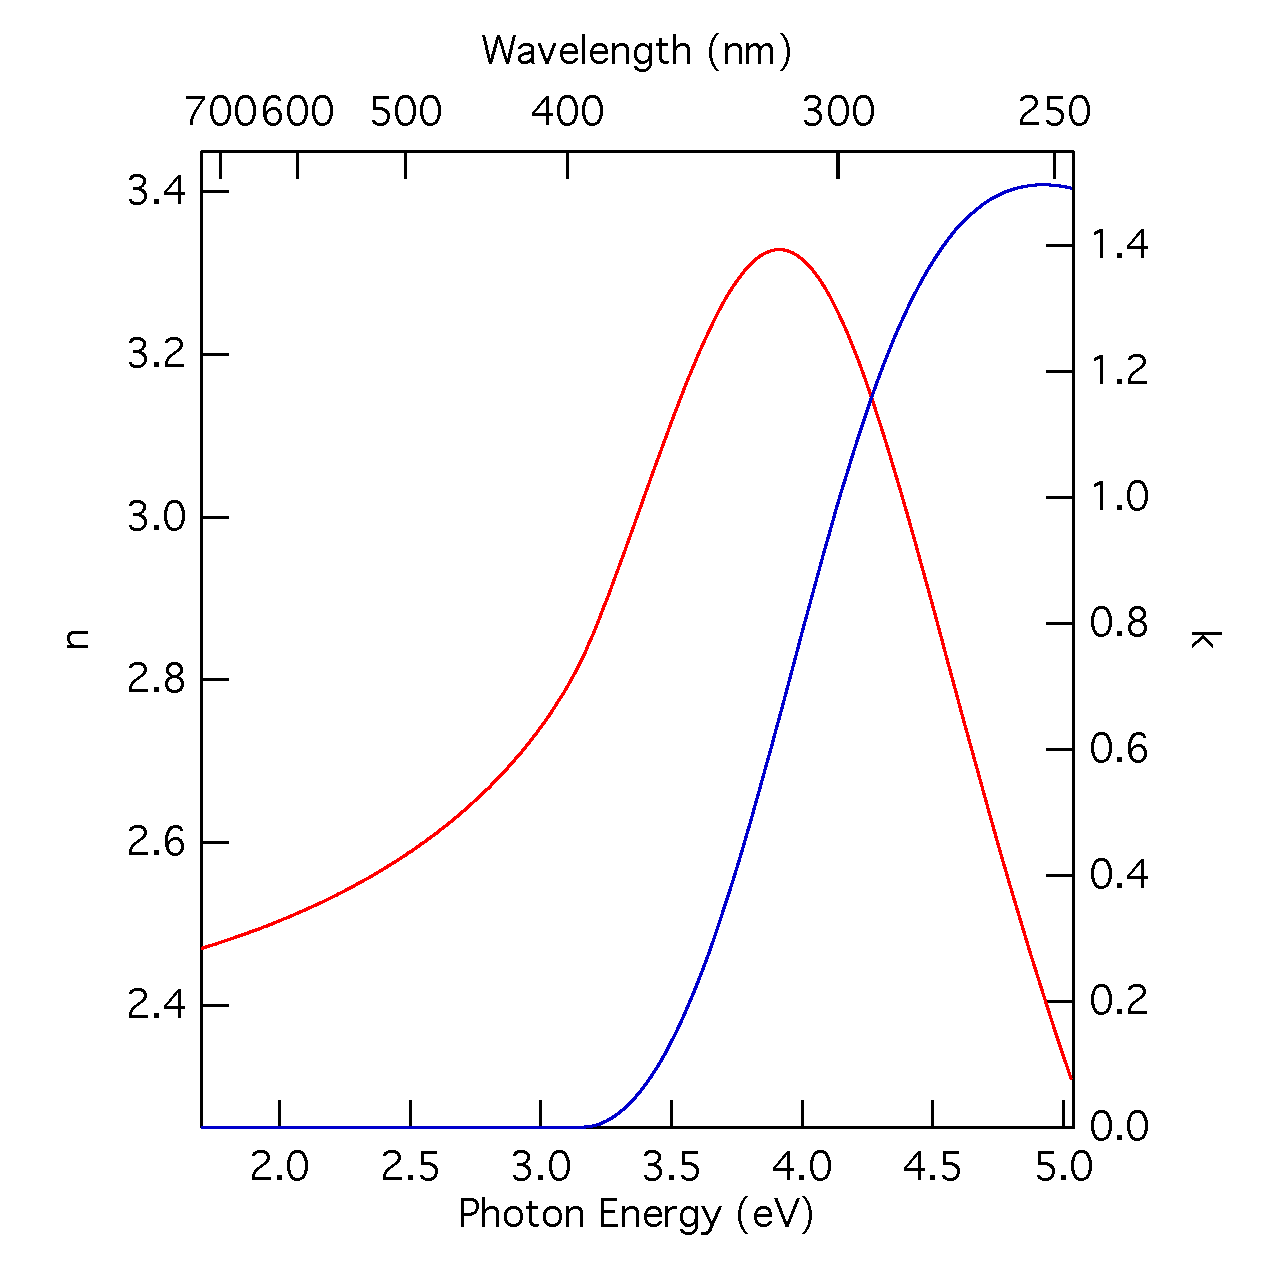
\includegraphics[width=0.47\textwidth]{./Figures/Appendix/Ellipsometry/Run-0-SiO2/n,k.pdf}%
	}
   \caption[Results of Ellipsometry on Sample \#0]%
   		{The set of plots shown above show the results from ellipsometric analysis on sample \#0 (see %
		table~\vref{tbl:LoSamples}) grown on a silicon wafer and subsequently annealed. (a) and (b) %
		show the data and the modeled fit from the experiment. (c) shows the components of the complex %
		index of refraction ($\tilde n$), $n$ and $k$. Band gap estimation was performed using the values %
		of $k$. The highlighted portion of $k$ is the nearly linear region used in this analysis.}
   \label{fig:Ellip-0-SiO2}
\end{figure}

\begin{figure}[htbp]
   \centering
   \subfloat[Absorption ($\alpha$) vs. Photon Energy][Absorption ($\alpha$) vs. Photon Energy (eV)]{%
   	\label{fig:Ellip-0-SiO2-alpha}%
	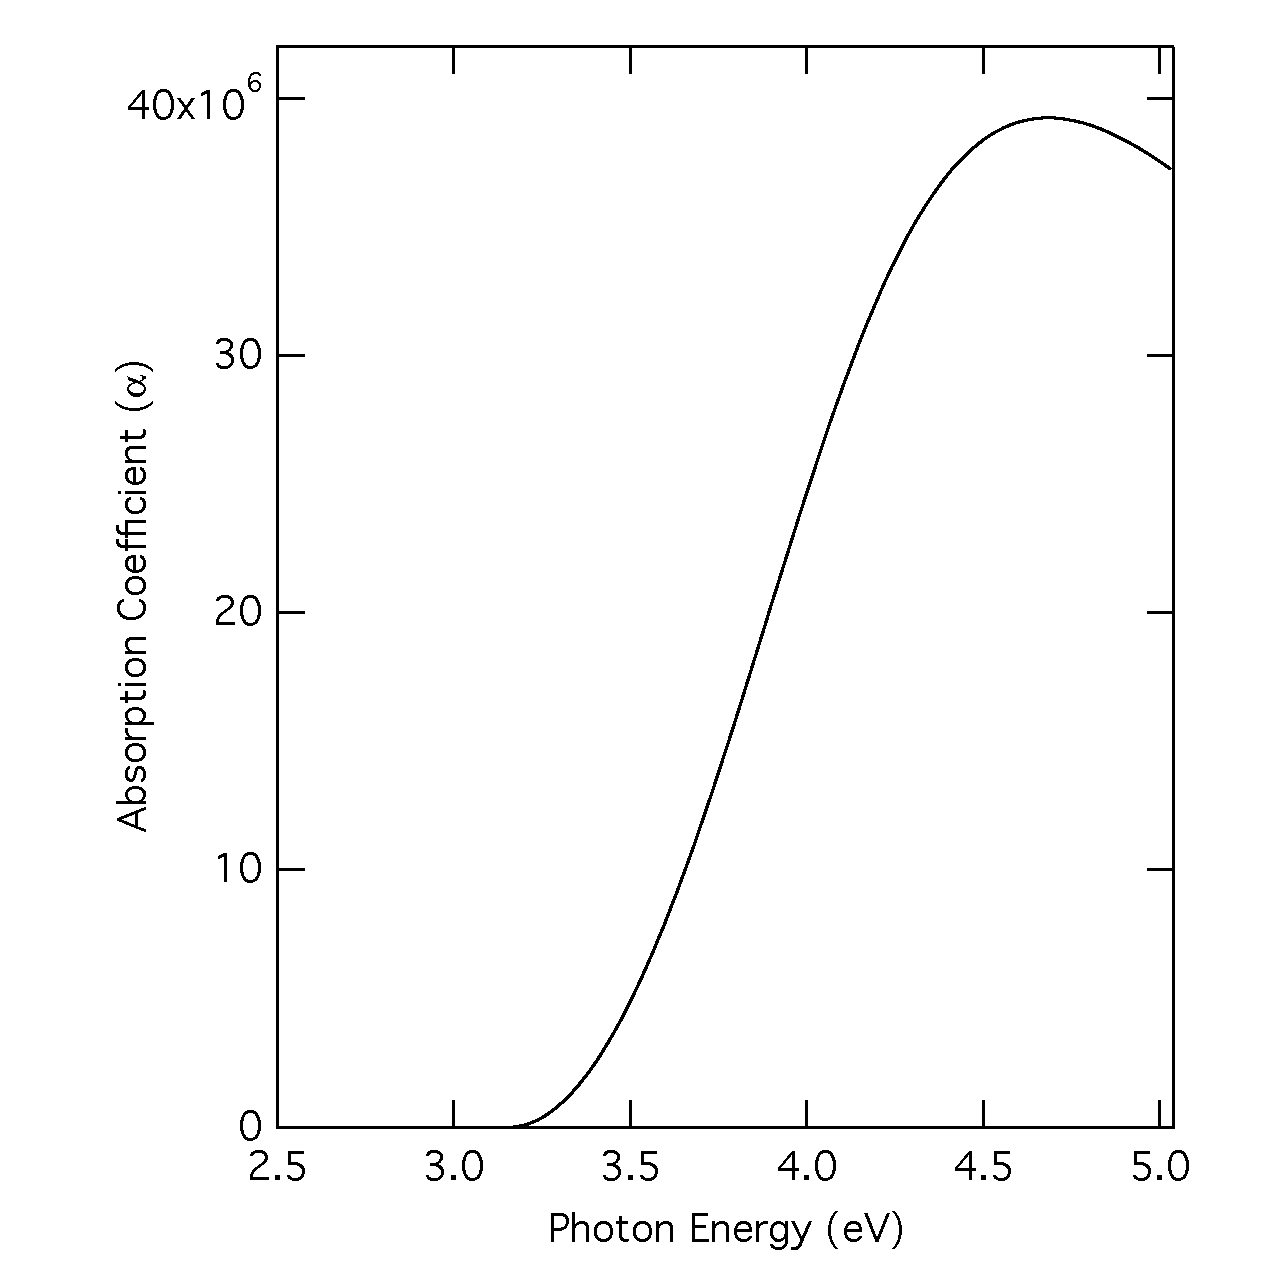
\includegraphics[width=0.47\textwidth]{./Figures/Appendix/Ellipsometry/Run-0-SiO2/alpha.pdf}%
	}\hspace{0.5cm}
  \subfloat[Tauc ($\alpha^{2}E_{ph}^{2}$) vs. Photon Energy][Tauc ($\alpha^{2}E_{ph}^{2}$) vs. Photon Energy (eV)]{%
   	\label{fig:Ellip-0-SiO2-Tauc}%
	\includegraphics[width=0.47\textwidth]{./Figures/Appendix/Ellipsometry/Run-0-SiO2/tauc.pdf}%
	}
   \caption[Results of Tauc Analysis on Sample \#0]%
   		{Tauc analysis used to determine the bandgap of PTO \#0. (a) shows the %
		values of the absorption coefficient ($\alpha$) calculated from $k$ (seen in figure~%
		\vref{fig:Ellip-0-SiO2-nk}). (b) shows the Tauc plot, the linear region can provide an estimate of the %
		bandgap of the material. }
   \label{fig:Tauc-0-SiO2}
\end{figure}

\begin{table}[htbp]
	\centering
	\caption[PTO \#20 Ellipsometric Model Variables]{Variables used to produce the\\model fit for PTO \#20 seen in fig.~\vref{fig:Ellip-20-Pt}. \label{tbl:PTO-20-ellip-variables}}
	\begin{tabular}{l l r r}
	\toprule
	Layer&Variable&Thickness (nm)&Value\\
	\midrule
	3. T-L Osc.&&75.6&\\
	&$\epsilon_{1}$ offset&&3.62\\
	&Amp&&36.54\\
	&E$_{\mathrm{n}}$&&4.51\\
	&C&&1.30\\
	&E$_{\mathrm{g}}$&&2.07\\
	2. \ce{Pt}&&15.1&\\
	1. \ce{SiO2}&& 1.1\\
	0. \ce{Si}&&Substrate&\\
	\bottomrule
	\end{tabular}
\end{table}

\begin{figure}[htbp]
   \centering
   \subfloat[Psi vs. Wavelength][Psi ($\Psi$) vs. Wavelength ($\lambda$)]{%
   	\label{fig:Ellip-20-Pt-Psi}%
	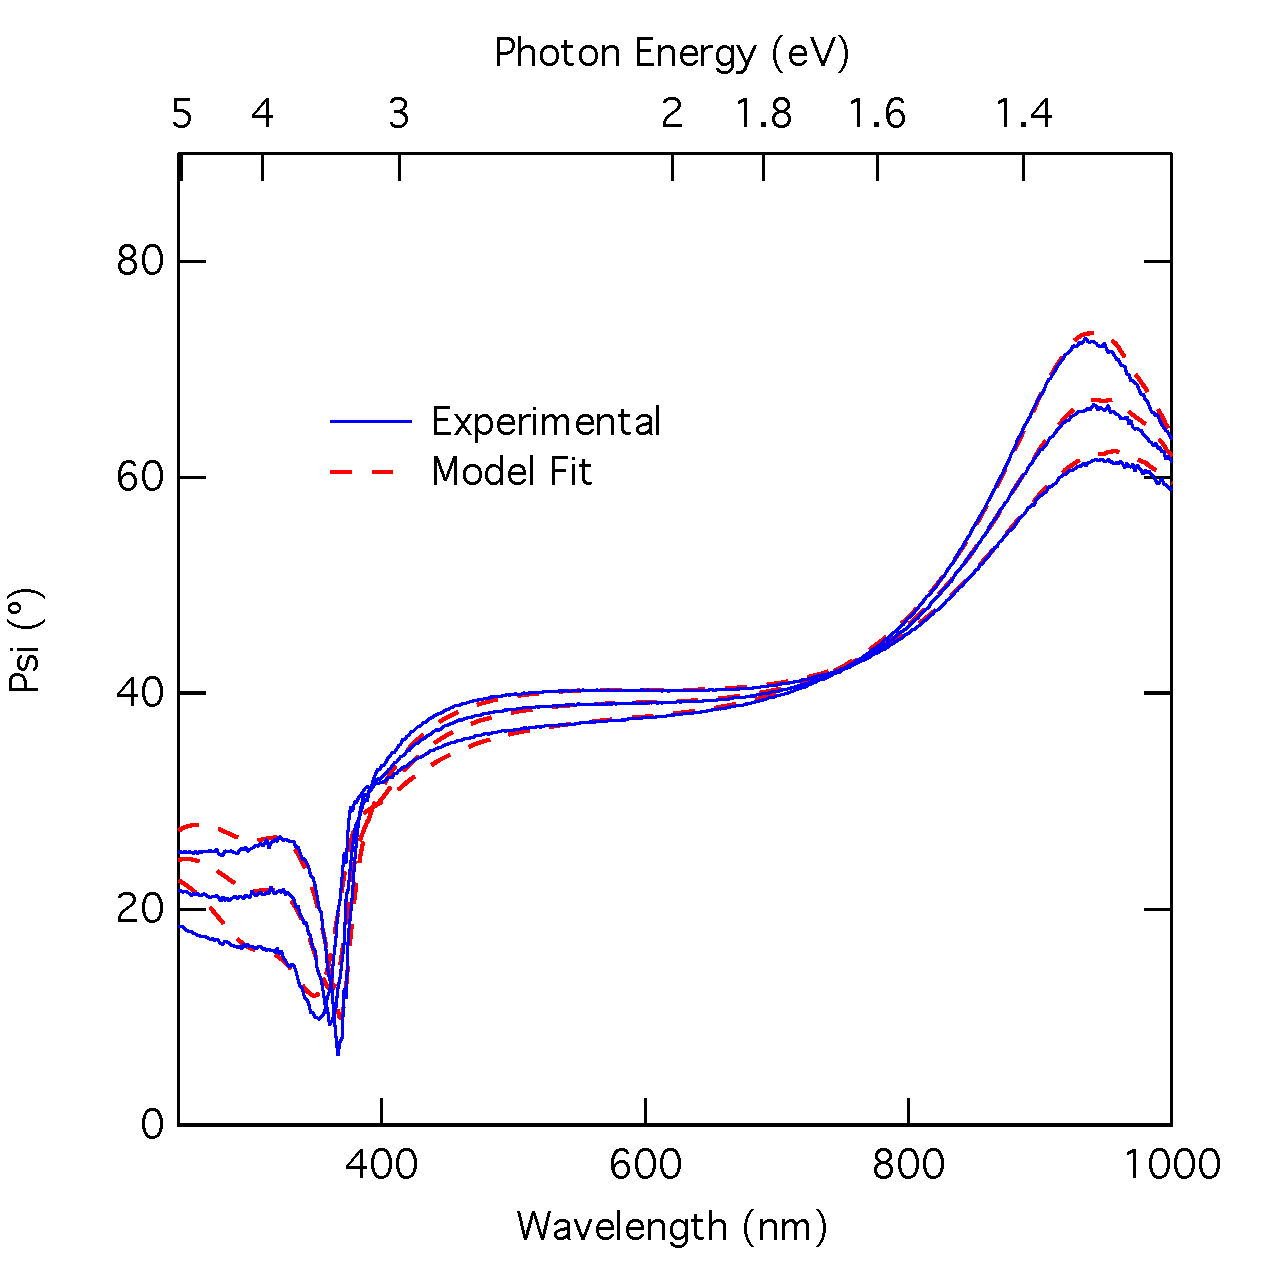
\includegraphics[width=0.47\textwidth]{./Figures/Appendix/Ellipsometry/Run-20-Pt/Psi.pdf}%
	}\hspace{0.5cm}
  \subfloat[Delta vs. Wavelength][Delta ($\Delta$) vs. Wavelength ($\lambda$)]{%
   	\label{fig:Ellip-20-Pt-Delta}%
	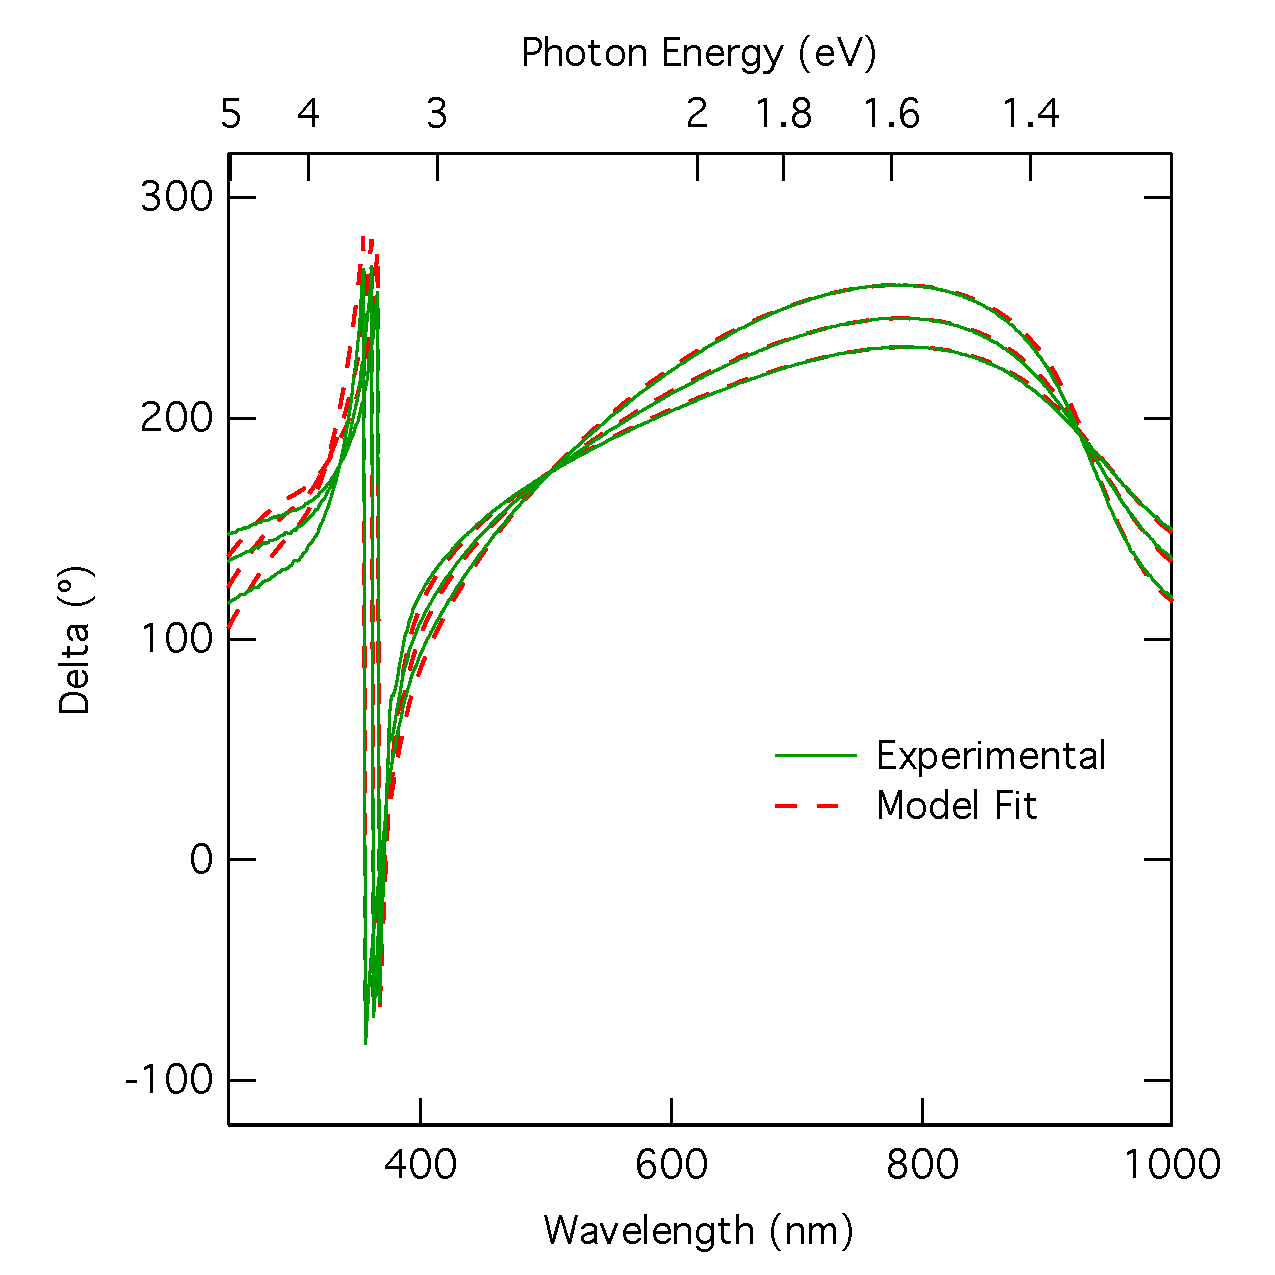
\includegraphics[width=0.47\textwidth]{./Figures/Appendix/Ellipsometry/Run-20-Pt/Delta.pdf}%
	} \\
  \subfloat[$n$, $k$ vs. Photon Energy][$n$, $k$ vs. Photon Energy (eV)]{%
   	\label{fig:Ellip-20-Pt-nk}%
	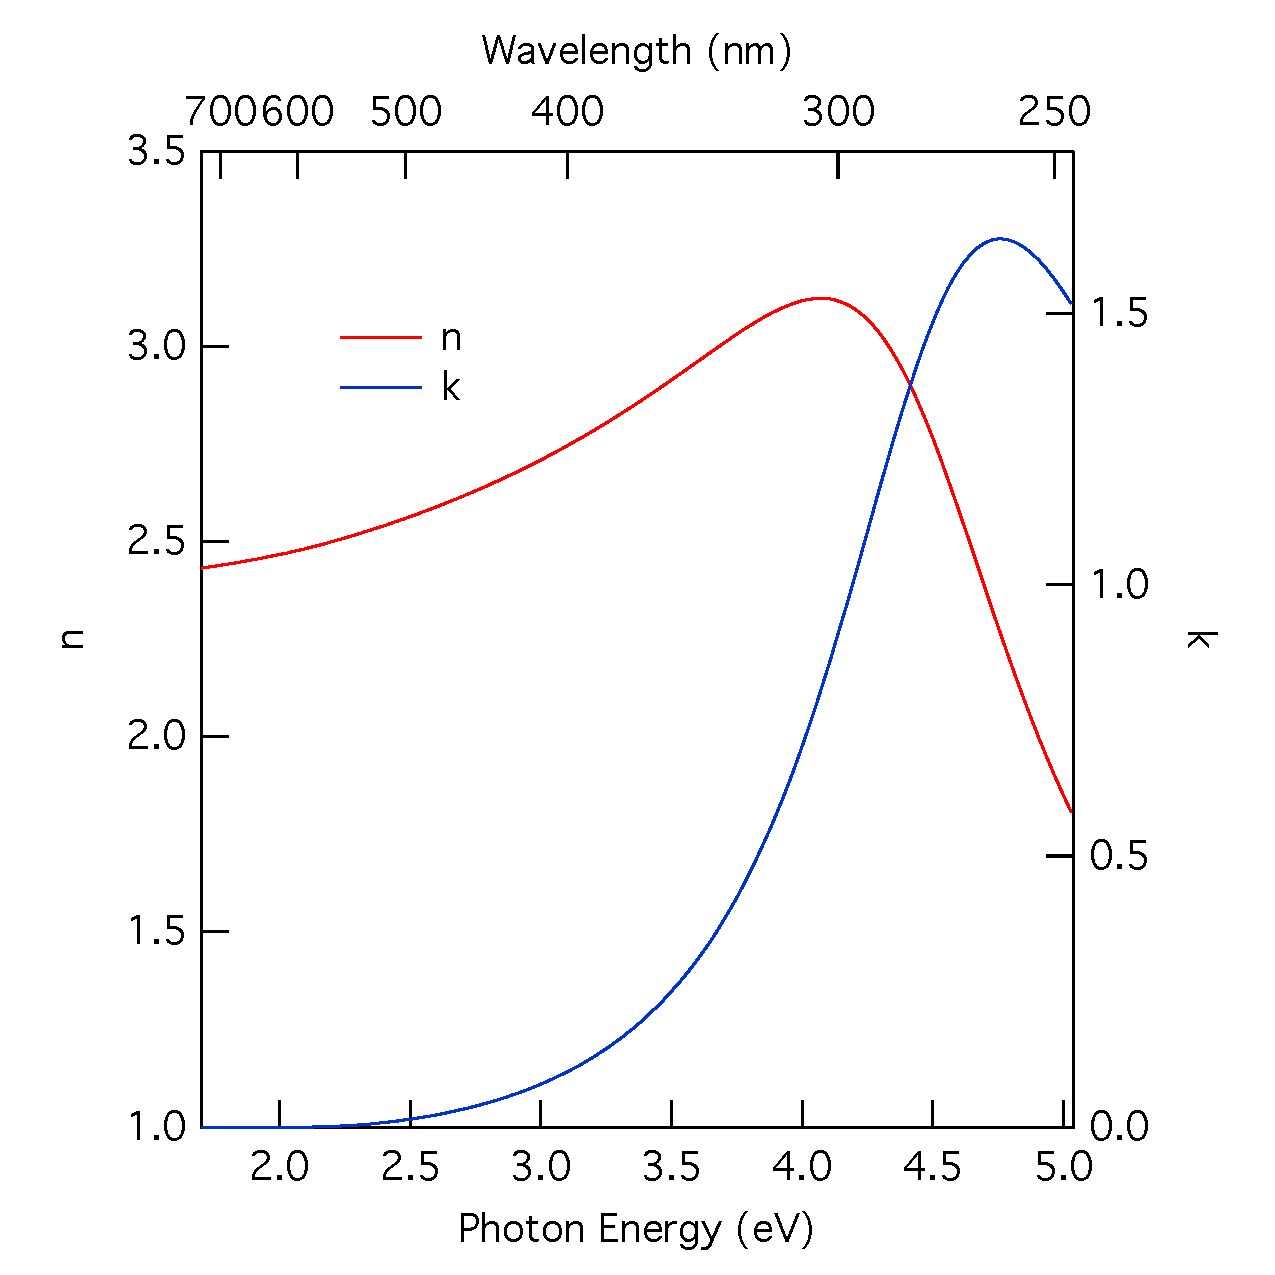
\includegraphics[width=0.47\textwidth]{./Figures/Appendix/Ellipsometry/Run-20-Pt/n,k.pdf}%
	}
   \caption[Results of Ellipsometry on Sample \#20 on Platinized Silicon]%
   		{Results of ellipsometric analysis on sample \#20, deposited on a platinized silicon substrate. As in fig.\ref{fig:Ellip-0-SiO2}, (a) and (b) show the experimental data and model fits of psi and delta (respectively). (c) gives the plot of calculated $n$ and $k$. For model parameters, see table~\vref{tbl:PTO-20-ellip-variables}}
		\label{fig:Ellip-20-Pt}
\end{figure}

\begin{figure}[htbp]
   \label{fig:Tauc-20-Pt}
   \centering
   \subfloat[Absorption ($\alpha$) vs. Photon Energy][Absorption ($\alpha$) vs. Photon Energy (eV)]{%
   	\label{fig:Ellip-20-Pt-alpha}%
	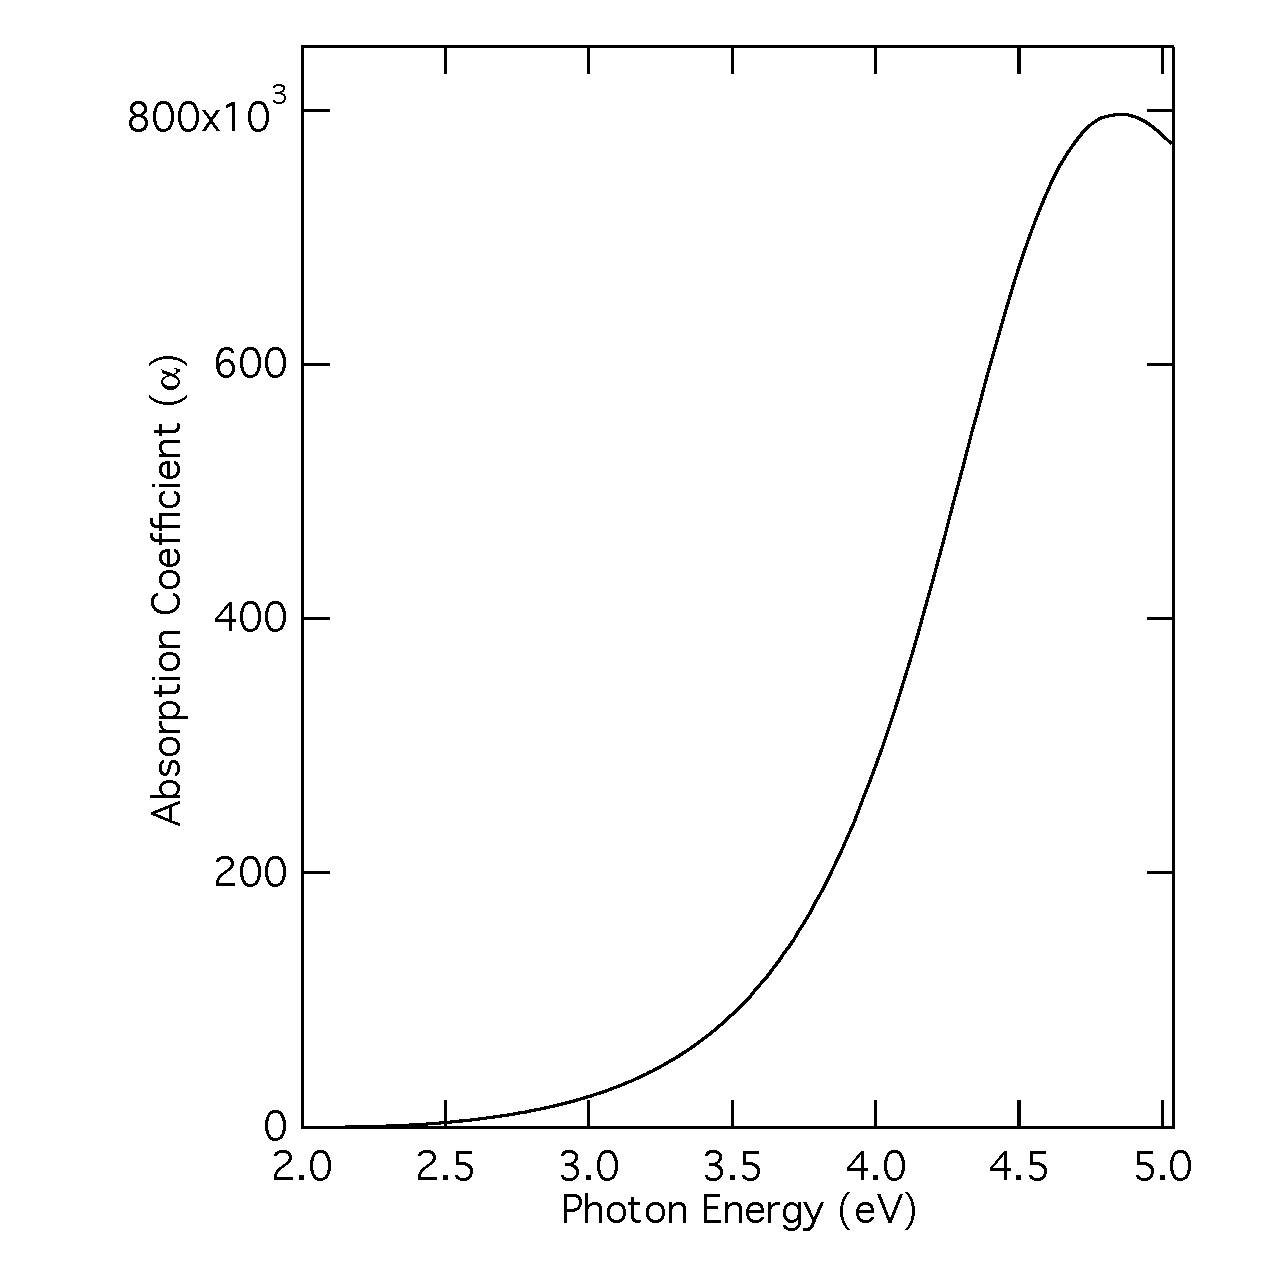
\includegraphics[width=0.47\textwidth]{./Figures/Appendix/Ellipsometry/Run-20-Pt/alpha.pdf}%
	}\hspace{0.5cm}
  \subfloat[Tauc ($\alpha^{2}E_{ph}^{2}$) vs. Photon Energy][Tauc ($\alpha^{2}E_{ph}^{2}$) vs. Photon Energy (eV)]{%
   	\label{fig:Ellip-20-Pt-Tauc}%
	\includegraphics[width=0.47\textwidth]{./Figures/Appendix/Ellipsometry/Run-20-Pt/tauc.pdf}%
	}
   \caption[Results of Tauc Analysis on Sample \#20 on Platinized Silicon]%
   		{Tauc analysis of sample \#20 on Pt-Si}
\end{figure}

\begin{table}[htbp]
	\centering
	\caption[PTO \#28 Ellipsometric Model Variables]{Variables used to produce the\\model fit for PTO \#28 seen in fig.~\vref{fig:Ellip-28-STO}. \label{tbl:PTO-28-ellip-variables}}
	\begin{tabular}{l l r r}
	\toprule
	Layer&Variable&Thickness (nm)&Value\\
	\midrule
	1. T-L Osc. (2)&&49.2&\\
	&$\epsilon_{1}$ offset&&1.42\\
	&Amp$_{1}$&&64.71\\
	&E$_{\mathrm{n 1}}$&&3.69\\
	&C$_{1}$&&4.44\\
	&E$_{\mathrm{g1}}$&&1.55\\
	&Amp$_{2}$&&1.55\\
	&E$_{\mathrm{n 2}}$&&2.12\\
	&C$_{2}$&&0.76\\
	&E$_{\mathrm{g2}}$&&0.001\\
	0. \ce{STO}&&Substrate&\\
	\bottomrule
	\end{tabular}
\end{table}

\begin{figure}[htbp]
   \centering
   \subfloat[Psi vs. Wavelength][Psi ($\Psi$) vs. Wavelength ($\lambda$)]{%
   	\label{fig:Ellip-28-STO-Psi}%
	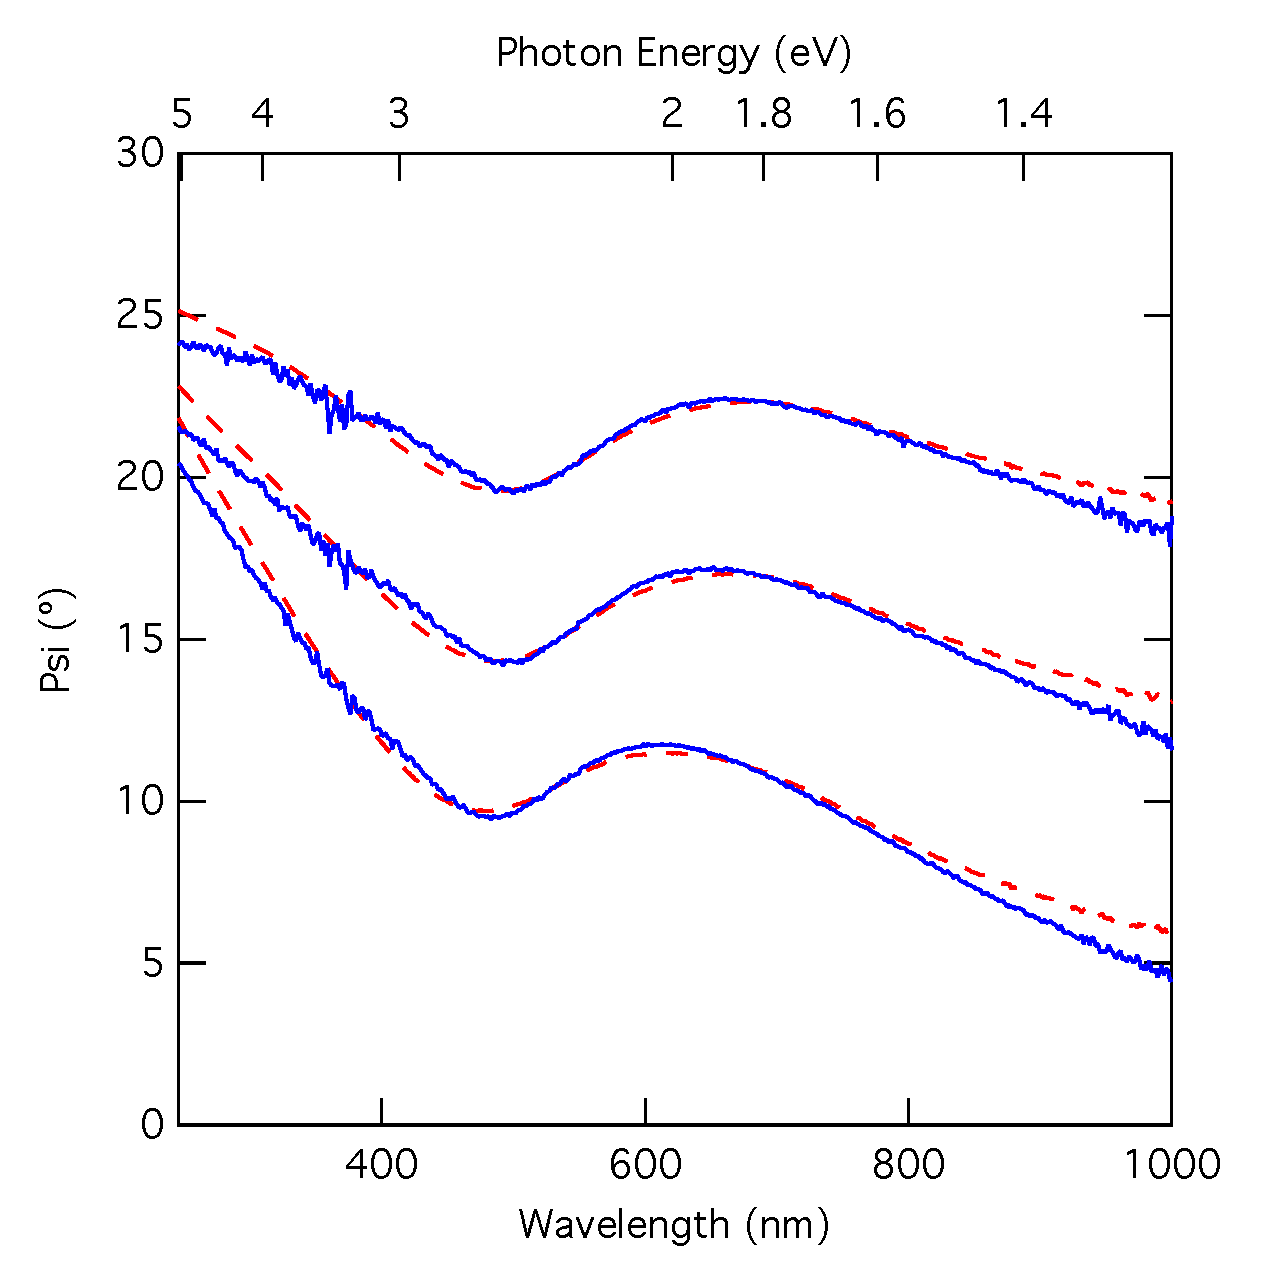
\includegraphics[width=0.47\textwidth]{./Figures/Appendix/Ellipsometry/Run-28-STO/Psi.pdf}%
	}\hspace{0.5cm}
  \subfloat[Delta vs. Wavelength][Delta ($\Delta$) vs. Wavelength ($\lambda$)]{%
   	\label{fig:Ellip-28-STO-Delta}%
	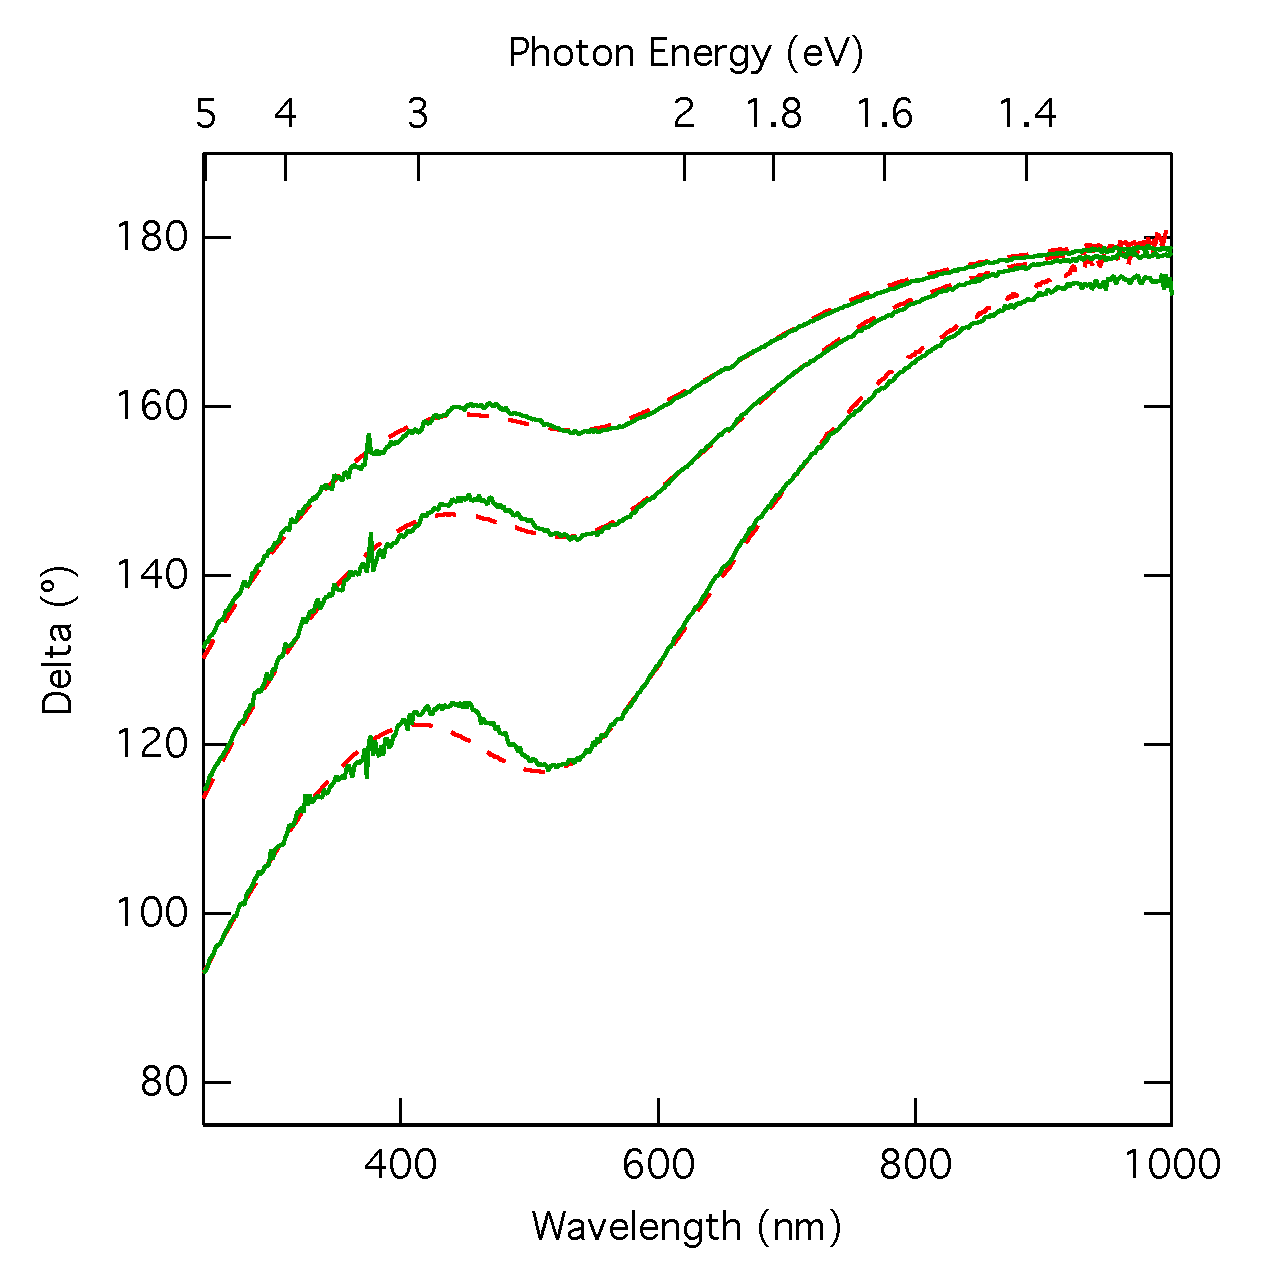
\includegraphics[width=0.47\textwidth]{./Figures/Appendix/Ellipsometry/Run-28-STO/Delta.pdf}%
	} \\
  \subfloat[$n$, $k$ vs. Photon Energy][$n$, $k$ vs. Photon Energy (eV)]{%
   	\label{fig:Ellip-28-STO-nk}%
	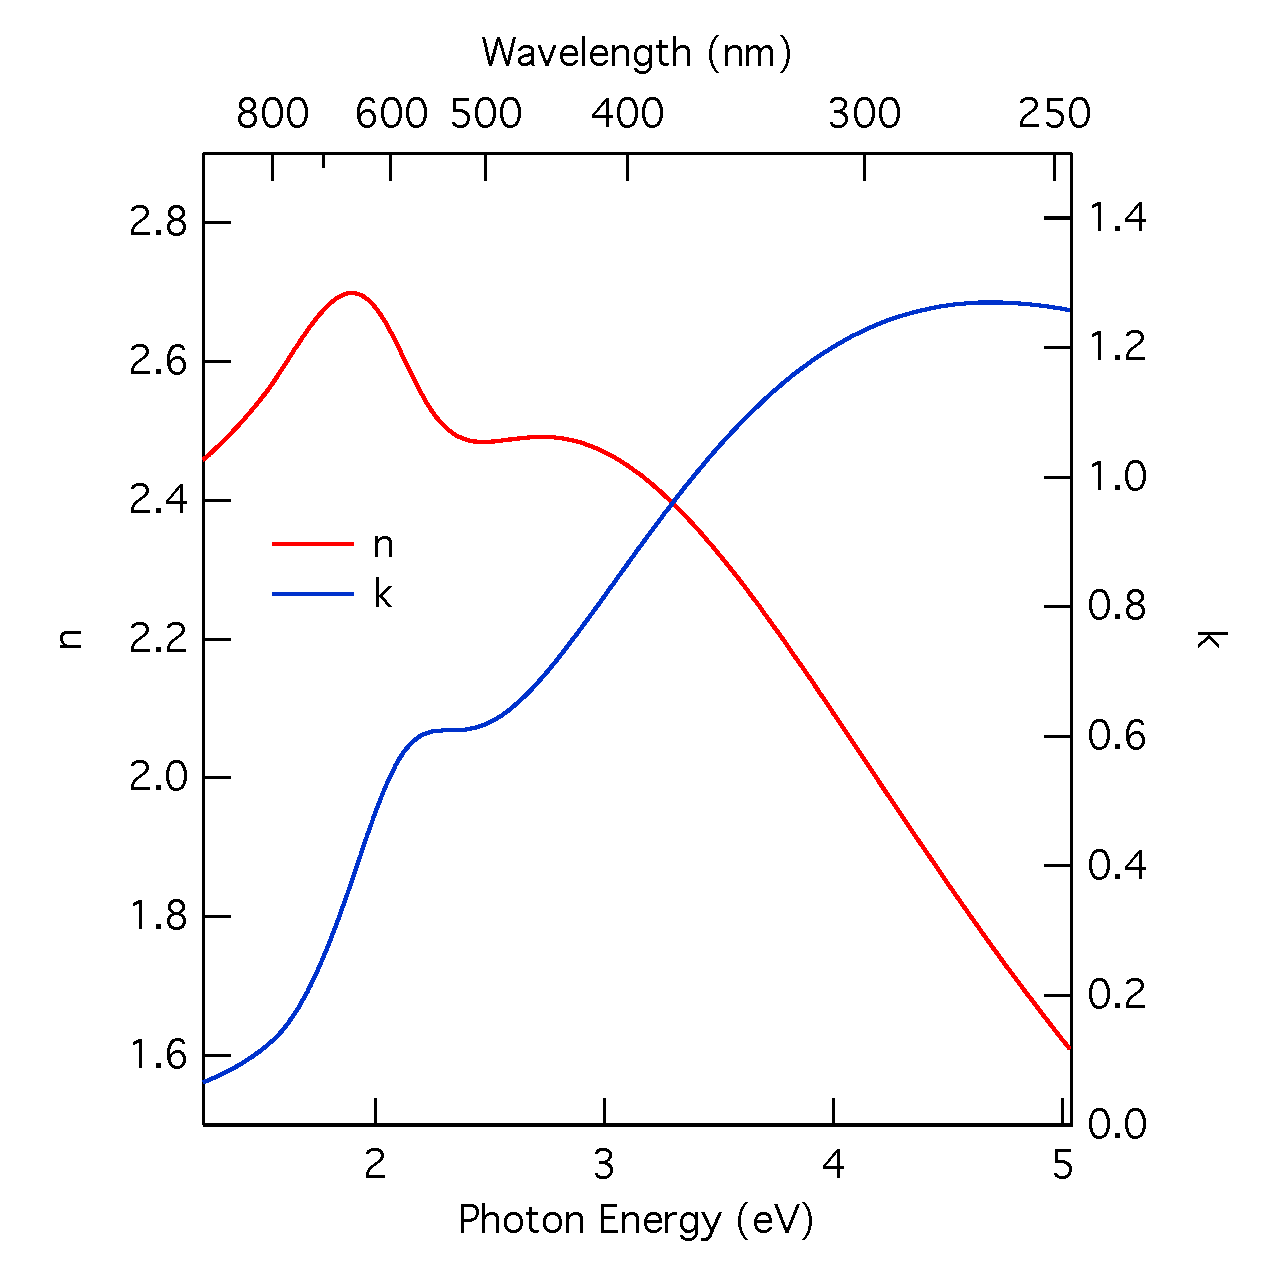
\includegraphics[width=0.47\textwidth]{./Figures/Appendix/Ellipsometry/Run-28-STO/n,k.pdf}%
	}
   \caption[Results of Ellipsometry on Sample \#28 on STO]%
   		{Results of ellipsometric analysis on sample \#28, deposited on a strontium titanate \ce{SrTiO3}(100) single crystalline substrate. As in fig.~\ref{fig:Ellip-0-SiO2}, (a) and (b) show the experimental data and model fits of psi and delta (respectively). (c) gives the plot of calculated $n$ and $k$.  This sample would not model well without a second oscillator, which gives rise to the secondary peaks in the $n$, $k$, and $\alpha$ plots (see fig.~\vref{fig:Ellip-28-STO-alpha}). For model parameters, see table~\vref{tbl:PTO-28-ellip-variables}.}
		\label{fig:Ellip-28-STO}
\end{figure}

\begin{figure}[htbp]
   \centering
   \subfloat[Absorption ($\alpha$) vs. Photon Energy][Absorption ($\alpha$) vs. Photon Energy (eV)]{%
   	\label{fig:Ellip-28-STO-alpha}%
	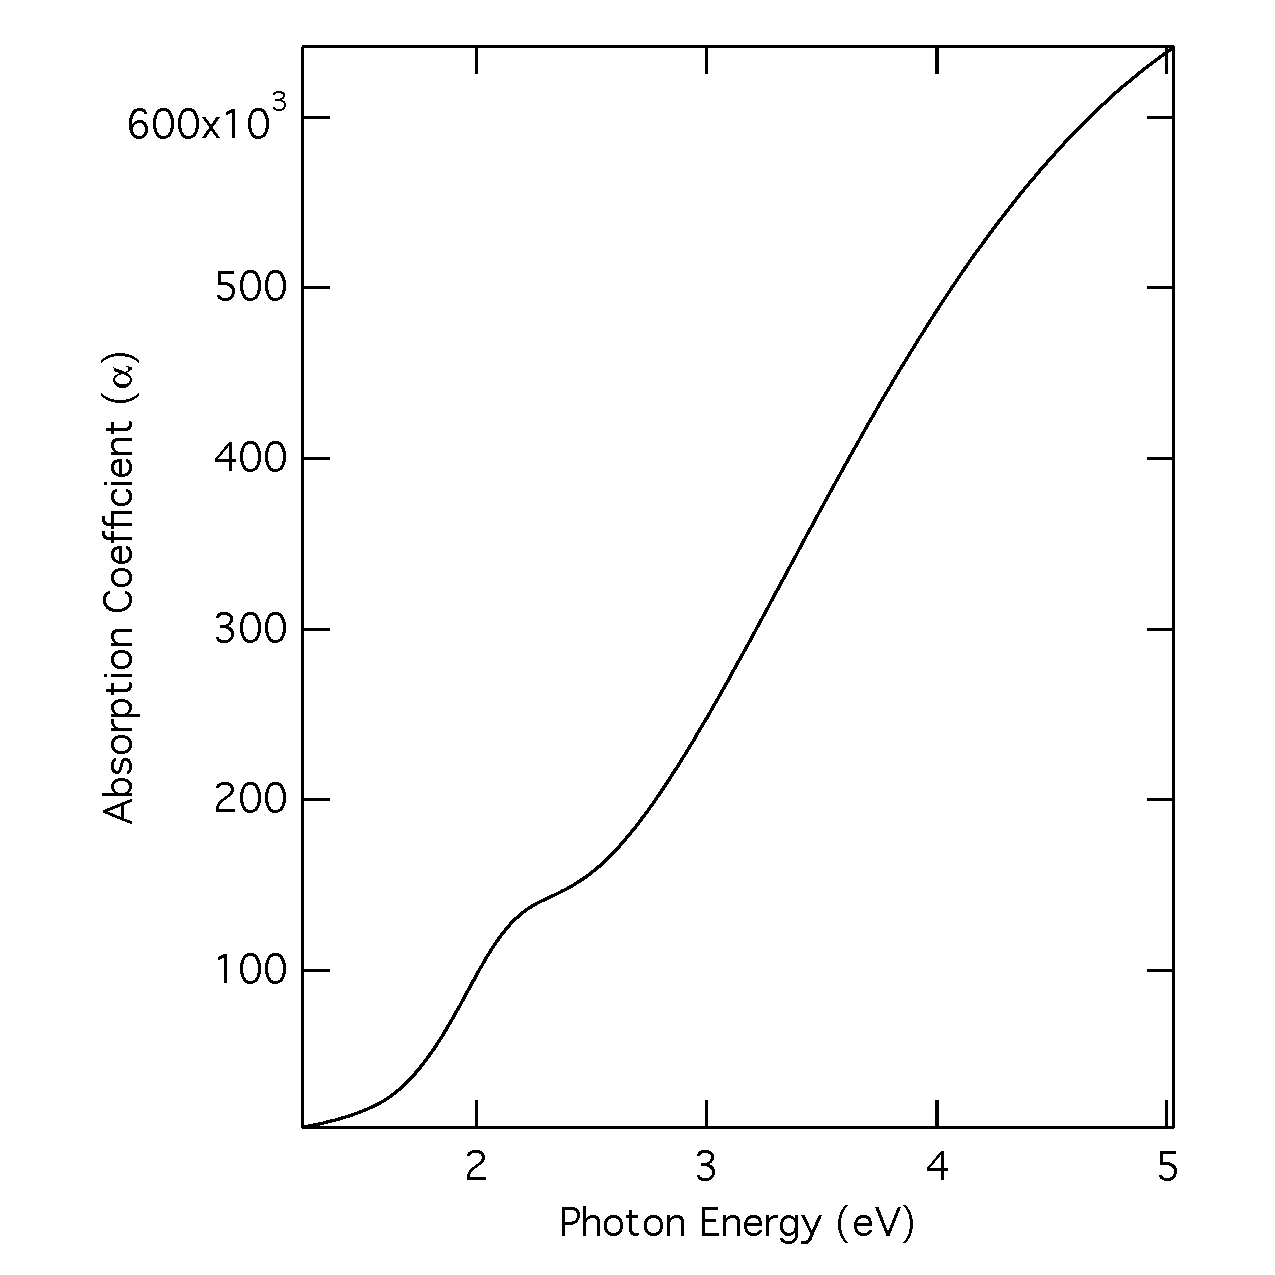
\includegraphics[width=0.47\textwidth]{./Figures/Appendix/Ellipsometry/Run-28-STO/alpha.pdf}%
	}\hspace{0.5cm}
  \subfloat[Tauc ($\alpha^{2}E_{ph}^{2}$) vs. Photon Energy][Tauc ($\alpha^{2}E_{ph}^{2}$) vs. Photon Energy (eV)]{%
   	\label{fig:Ellip-28-STO-Tauc}%
	\includegraphics[width=0.47\textwidth]{./Figures/Appendix/Ellipsometry/Run-28-STO/tauc.pdf}%
	}
   \caption[Results of Tauc Analysis on Sample \#28 on STO]%
   		{Eg = 3.506. Tauc analysis of sample \#28 - STO. Notice that the second oscillator can be seen in the absorption coefficient (a), but does not affect the shape of the Tauc plot (b) and thus does not interfere with bandgap estimation.}\label{fig:Tauc-28-STO}
\end{figure}

\begin{table}
	\centering
	\caption[Calculated Band Gap Energies]{Band gap energies, determined via Tauc analysis of ellipsometric data}%
	\label{tbl:bandgaps}
	\begin{tabular}{l l r}
		\toprule
		Run \#	&Subs. Type	&Band Gap (eV)\\ \midrule
		0		&Si			&3.763\\
		20		&Pt-Si		&4.058\\
		28		&STO		&3.506\\
		\bottomrule
	\end{tabular}
\end{table}

\clearpage
%%%%%%%%%%%%%%%%%%%%%%%%%%%%%%%%%%%%%%%%%%%%%%%%%%%%
%%%%%%%%%%%%%%%%%%%%%%%%%%%%%%%%%%%%%%%%%%%%%%%%%%%%
%%%%%%%%%%%%%%%%%%%%%%%%%%%%%%%%%%%%%%%%%%%%%%%%%%%%

\section{XRD Results}
\label{sup:XRD}

\begin{figure}[htbp]
   \label{fig:XRD-20-Pt}
   \centering
   \subfloat[Full Range][Full Range Scan]{%
   	\label{fig:Ellip-20-Pt-20-50}%
	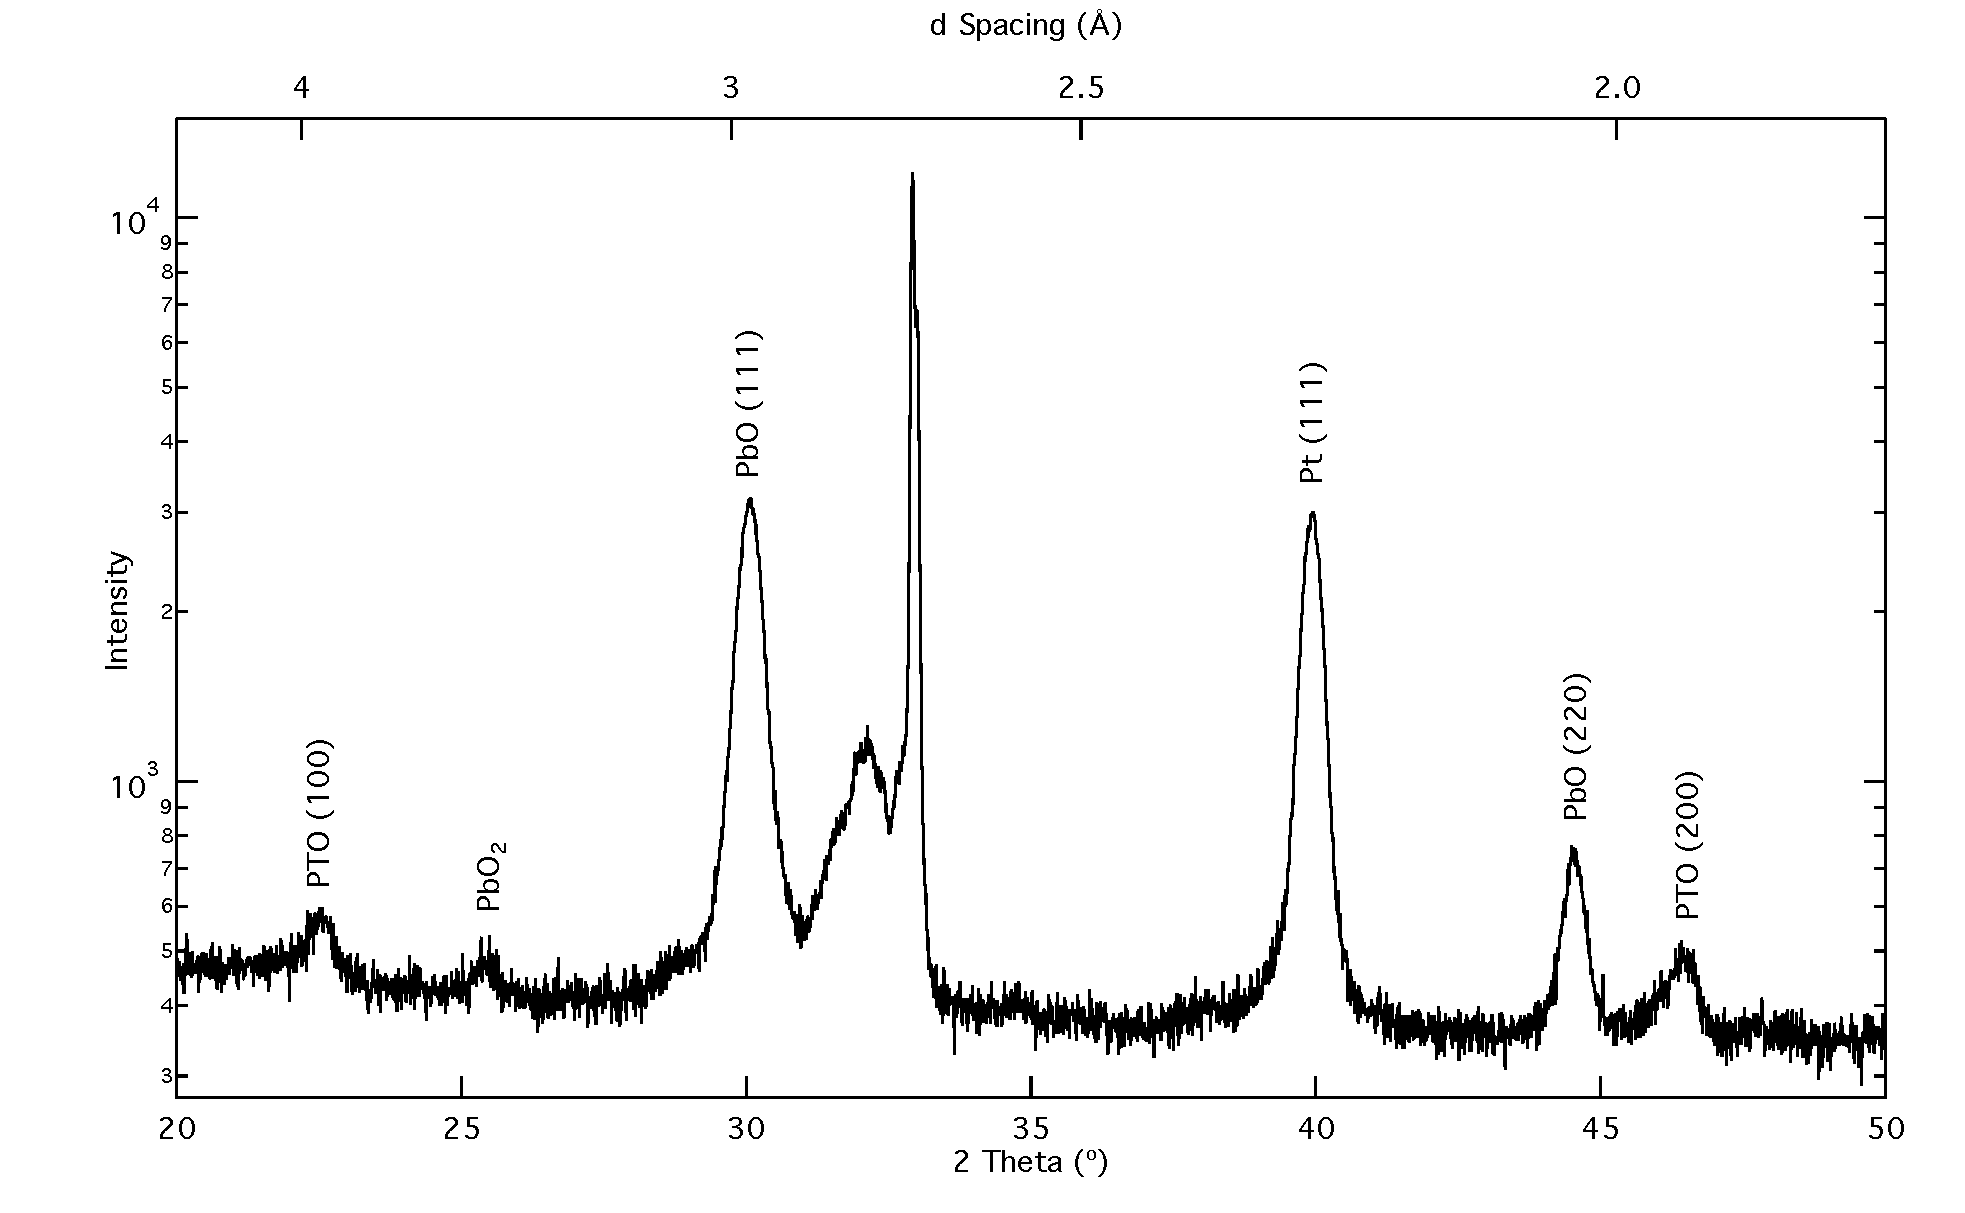
\includegraphics[width=0.95\textwidth]{./Figures/Appendix/XRD/Run-20-Pt/20-50.pdf}%
	}\\
  \subfloat[PTO (100) and PbO$_{2}$][PTO (100) and PbO$_{2}$]{%
   	\label{fig:XRD-20-Pt-20-27}%
	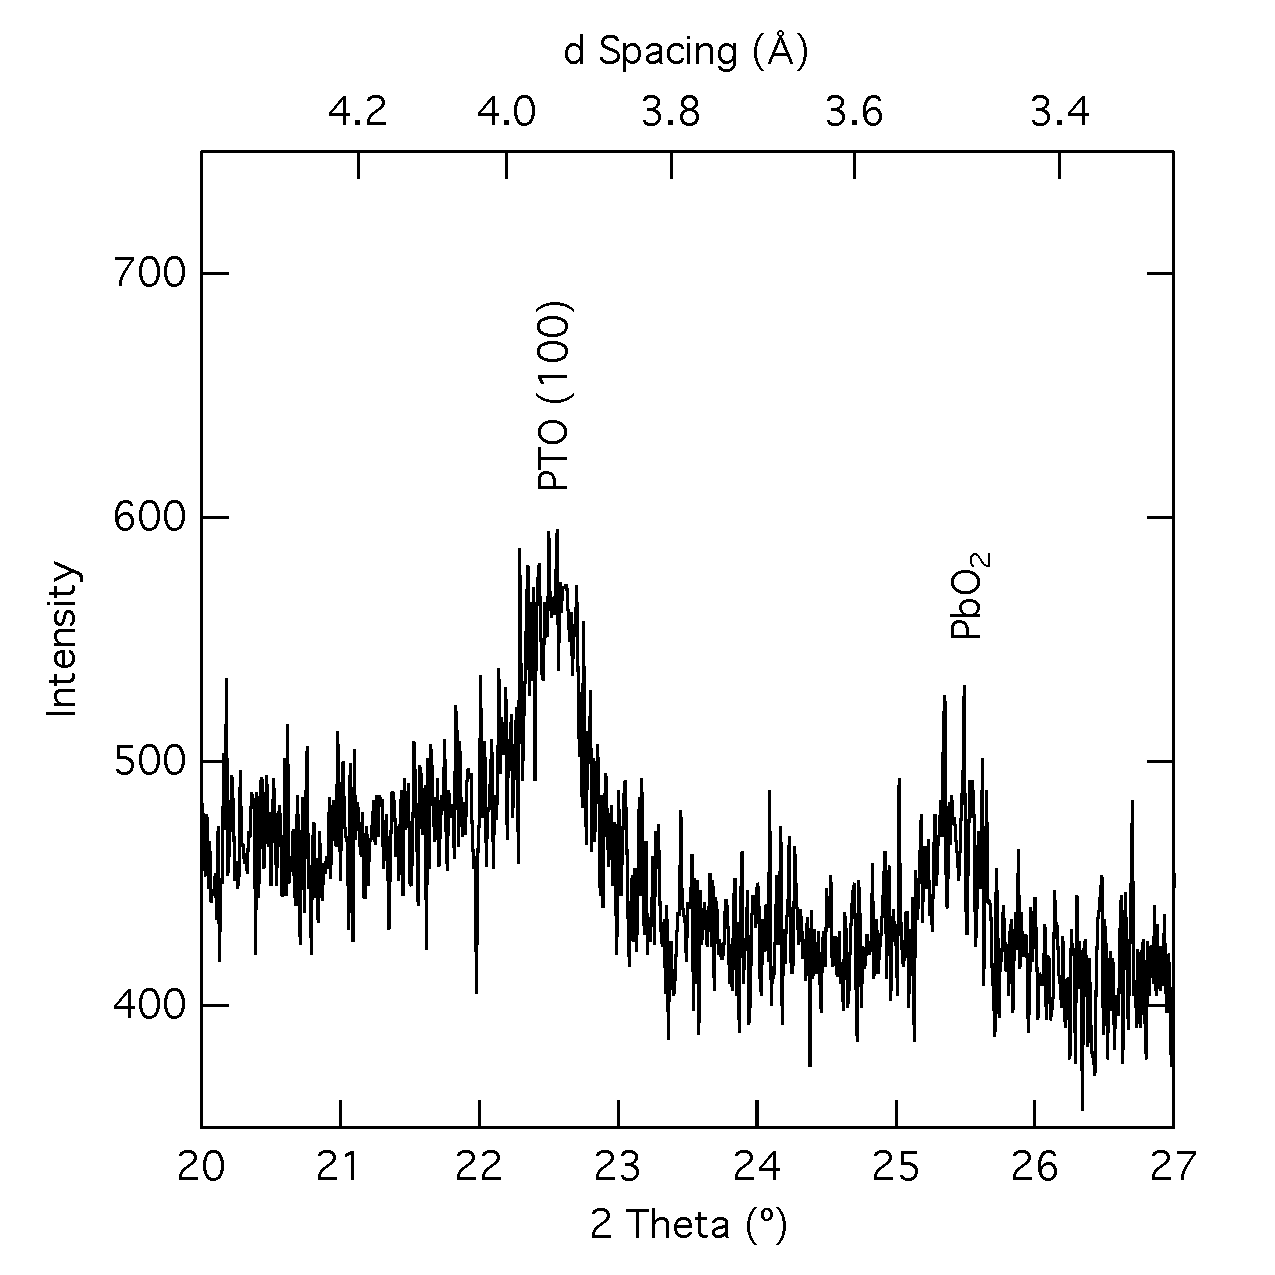
\includegraphics[width=0.47\textwidth]{./Figures/Appendix/XRD/Run-20-Pt/20-27.pdf}%
	} \hspace{0.5cm}
  \subfloat[PbO (220) and PTO (200)][PbO (220) and PTO (200)]{%
   	\label{fig:XRD-20-Pt-43-48}%
	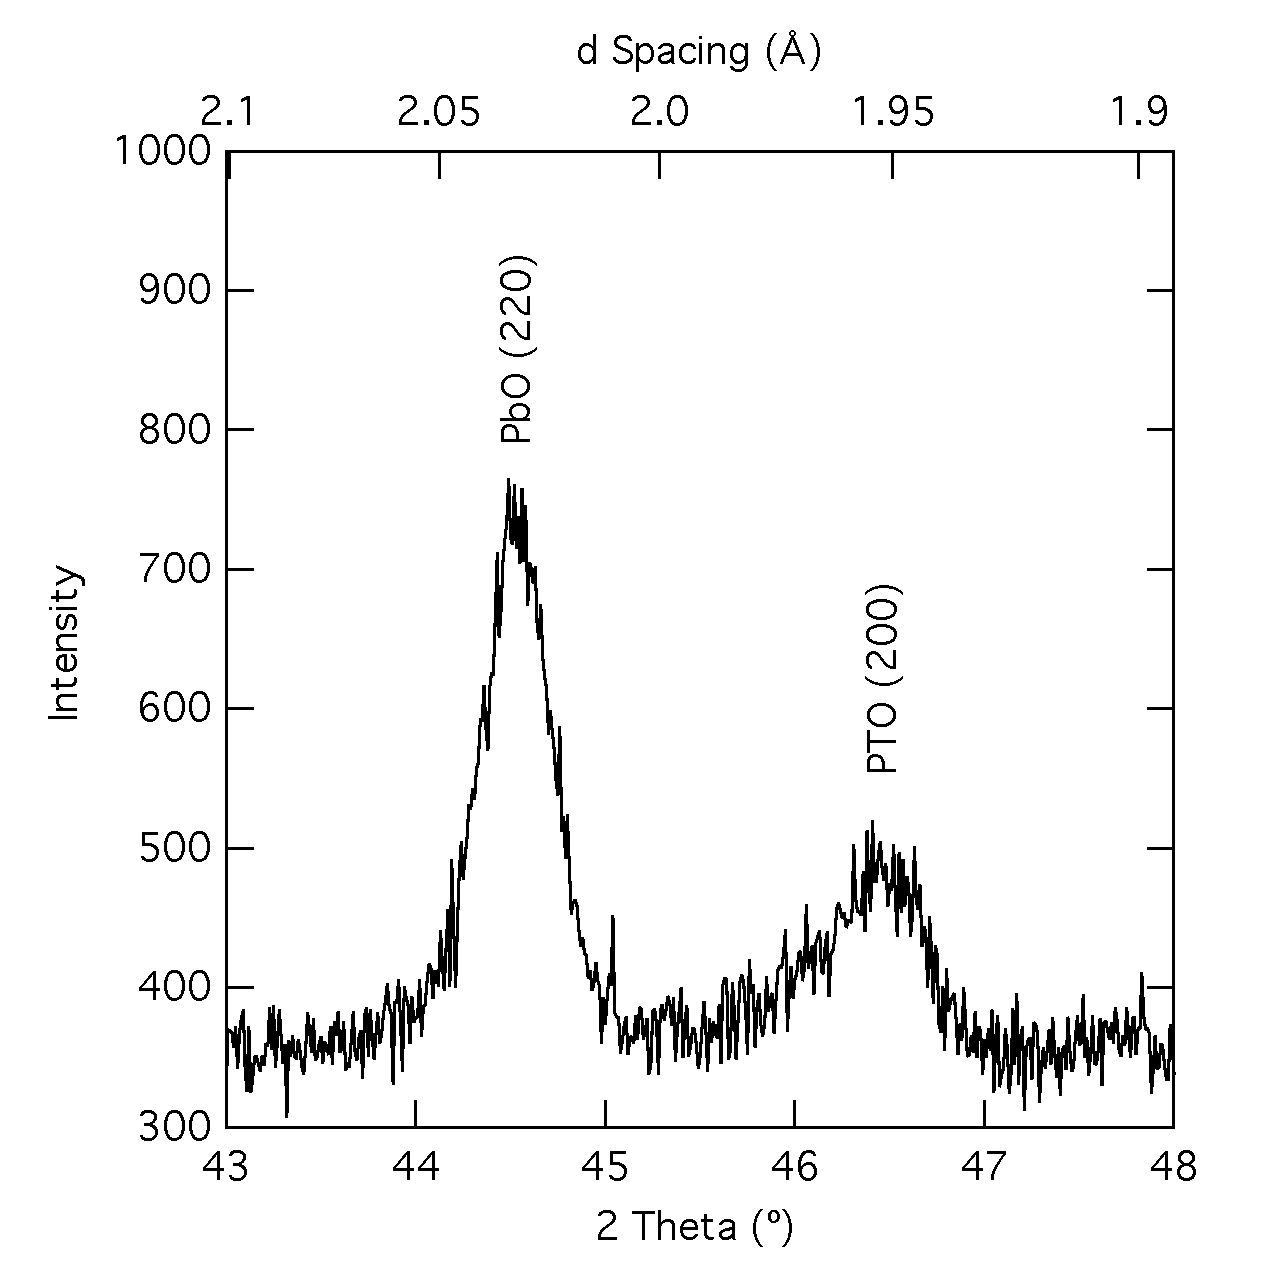
\includegraphics[width=0.47\textwidth]{./Figures/Appendix/XRD/Run-20-Pt/43-48.pdf}%
	}
   \caption[Results of XRD Experiments on Sample \#20 on Platinized Silicon]%
   		{XRD of \#20 Pt}
\end{figure}










\clearpage


























